%%%%%%%%%%%%%%%%%%%%%%%%%%%%%%%%%%%%%%%%%
% Short Sectioned Assignment LaTeX Template Version 1.0 (5/5/12)
% This template has been downloaded from: http://www.LaTeXTemplates.com
% Original author:  Frits Wenneker (http://www.howtotex.com)
% License: CC BY-NC-SA 3.0 (http://creativecommons.org/licenses/by-nc-sa/3.0/)
%%%%%%%%%%%%%%%%%%%%%%%%%%%%%%%%%%%%%%%%%

% \documentclass[paper=a4, fontsize=11pt]{scrartcl} % A4 paper and 11pt font size
\documentclass[11pt, a4paper]{book}
\usepackage[T1]{fontenc} % Use 8-bit encoding that has 256 glyphs
\usepackage[utf8]{inputenc}
\usepackage{fourier} % Use the Adobe Utopia font for the document - comment this line to return to the LaTeX default
\usepackage{listings} % para insertar código con formato similar al editor
\usepackage[spanish, es-tabla]{babel} % Selecciona el español para palabras introducidas automáticamente, p.ej. "septiembre" en la fecha y especifica que se use la palabra Tabla en vez de Cuadro
\usepackage{url} % ,href} %para incluir URLs e hipervínculos dentro del texto (aunque hay que instalar href)
\usepackage{graphics,graphicx, float} %para incluir imágenes y colocarlas
\usepackage[gen]{eurosym} %para incluir el símbolo del euro
\usepackage{cite} %para incluir citas del archivo <nombre>.bib
\usepackage{enumerate}
\usepackage{hyperref}
\usepackage{graphicx}
\usepackage{tabularx}
\usepackage{booktabs}
\usepackage[titletoc]{appendix}

\usepackage[table,xcdraw]{xcolor}
\hypersetup{
	colorlinks=true,	% false: boxed links; true: colored links
	linkcolor=black,	% color of internal links
	urlcolor=cyan		% color of external links
}
\renewcommand{\familydefault}{\sfdefault}
\usepackage{fancyhdr} % Custom headers and footers
\pagestyle{fancyplain} % Makes all pages in the document conform to the custom headers and footers
\fancyhead[L]{} % Empty left header
\fancyhead[C]{} % Empty center header
\fancyhead[R]{Víctor Cabrita Gómez} % My name
\fancyfoot[L]{} % Empty left footer
\fancyfoot[C]{} % Empty center footer
\fancyfoot[R]{\thepage} % Page numbering for right footer
%\renewcommand{\headrulewidth}{0pt} % Remove header underlines
\renewcommand{\footrulewidth}{0pt} % Remove footer underlines
\setlength{\headheight}{13.6pt} % Customize the height of the header

\usepackage{titlesec, blindtext, color}
\definecolor{gray75}{gray}{0.75}
\newcommand{\hsp}{\hspace{20pt}}
\titleformat{\chapter}[hang]{\Huge\bfseries}{\thechapter\hsp\textcolor{gray75}{|}\hsp}{0pt}{\Huge\bfseries}
\setcounter{secnumdepth}{4}
\usepackage[Lenny]{fncychap}


\begin{document}

	% Plantilla portada UGR
	\begin{titlepage}
\newlength{\centeroffset}
\setlength{\centeroffset}{-0.5\oddsidemargin}
\addtolength{\centeroffset}{0.5\evensidemargin}
\thispagestyle{empty}

\noindent\hspace*{\centeroffset}\begin{minipage}{\textwidth}

\centering

\includegraphics[width=0.9\textwidth]{logos/logo_ugr.jpg}\\[1.4cm]

\textsc{ \Large TRABAJO FIN DE GRADO\\[0.2cm]}
\textsc{ GRADO EN INGENIERÍA INFORMÁTICA}\\[1cm]

{\Huge\bfseries Título \\}
\noindent\rule[-1ex]{\textwidth}{3pt}\\[3.5ex]
{\large\bfseries Subtítulo }
\end{minipage}

\vspace{2.5cm}
\noindent\hspace*{\centeroffset}
\begin{minipage}{\textwidth}
\centering

\textbf{Autor}\\ {Estudiante}\\[2.5ex]
\textbf{Director}\\ {Tutor(a)(es)}\\[2cm]

\includegraphics[width=0.3\textwidth]{logos/etsiit_logo.png}\\[0.1cm]
\textsc{Escuela Técnica Superior de Ingenierías Informática y de Telecomunicación}\\
\textsc{---}\\
Granada, Junio de 201x
\end{minipage}
\end{titlepage}


	% Plantilla prefacio UGR
	\thispagestyle{empty}

\begin{center}
{\large\bfseries Título \\ Subtítulo }\\
\end{center}
\begin{center}
Nombre Del Estudiante\\
\end{center}

%\vspace{0.7cm}

\vspace{0.5cm}
\noindent{\textbf{Palabras clave}: \textit{software libre}
\vspace{0.7cm}

\noindent{\textbf{Resumen}\\
	

\cleardoublepage

\begin{center}
	{\large\bfseries Same, but in English}\\
\end{center}
\begin{center}
	Student's name\\
\end{center}
\vspace{0.5cm}
\noindent{\textbf{Keywords}: \textit{open source}, \textit{floss}
\vspace{0.7cm}

\noindent{\textbf{Abstract}\\


\cleardoublepage

\thispagestyle{empty}

\noindent\rule[-1ex]{\textwidth}{2pt}\\[4.5ex]

D. \textbf{Tutora/e(s)}, Profesor(a) del ...

\vspace{0.5cm}

\textbf{Informo:}

\vspace{0.5cm}

Que el presente trabajo, titulado \textit{\textbf{Chief}},
ha sido realizado bajo mi supervisión por \textbf{Estudiante}, y autorizo la defensa de dicho trabajo ante el tribunal
que corresponda.

\vspace{0.5cm}

Y para que conste, expiden y firman el presente informe en Granada a Junio de 2018.

\vspace{1cm}

\textbf{El/la director(a)/es: }

\vspace{5cm}

\noindent \textbf{(nombre completo tutor/a/es)}

\chapter*{Agradecimientos}






	% Índice de contenidos
	\newpage
	\tableofcontents

	% Índice de imágenes y tablas
	\newpage
	\listoffigures

	% Si hay suficientes se incluirá dicho índice
	\listoftables 
	\newpage

	% Introducción 
	\chapter{Introducción}

Este proyecto es software libre, y está liberado con la licencia General Public License v3 \cite{gplv3}.

\section{Motivación}
Con la irrupción y popularidad de diferentes servicios de streaming como Netflix \cite{Netflix} o HBO \cite{HBO}, el catálogo de series que uno puede ver ya no se limita a las que echen por la televisión. Ante este vasto mar de opciones, surgen dos problemas:
\begin{enumerate}
    \item Con tantas opciones, no somos capaces de discernir las que nos podrían interesar, causando el efecto contrario, que nos pasemos horas buscando para al final no ver nada.
    \item Como seres sociales que somos, nos surge la imperiosa necesidad de saber qué series se han visto nuestros conocidos y conocer su opinión sobre las mismas, a la vez que contarles a ellos nuestra opinión sobre las que nos hemos visto.
\end{enumerate}

El primer problema es resuelto en cierta forma por webs que clasifican y/o puntúan las series del catálogo actual. El segundo, a día de hoy sigue sin ser resuelto y está más que demostrada su necesidad por los usuarios de Twitter \cite{Twitter}, en los innumerables hilos en los que exponen su opinión sobre las series que han visto a lo largo del año.
\begin{figure}[H]
	\centering	
	
\includegraphics[scale=0.25]{img/twitter-thread-1.png}
    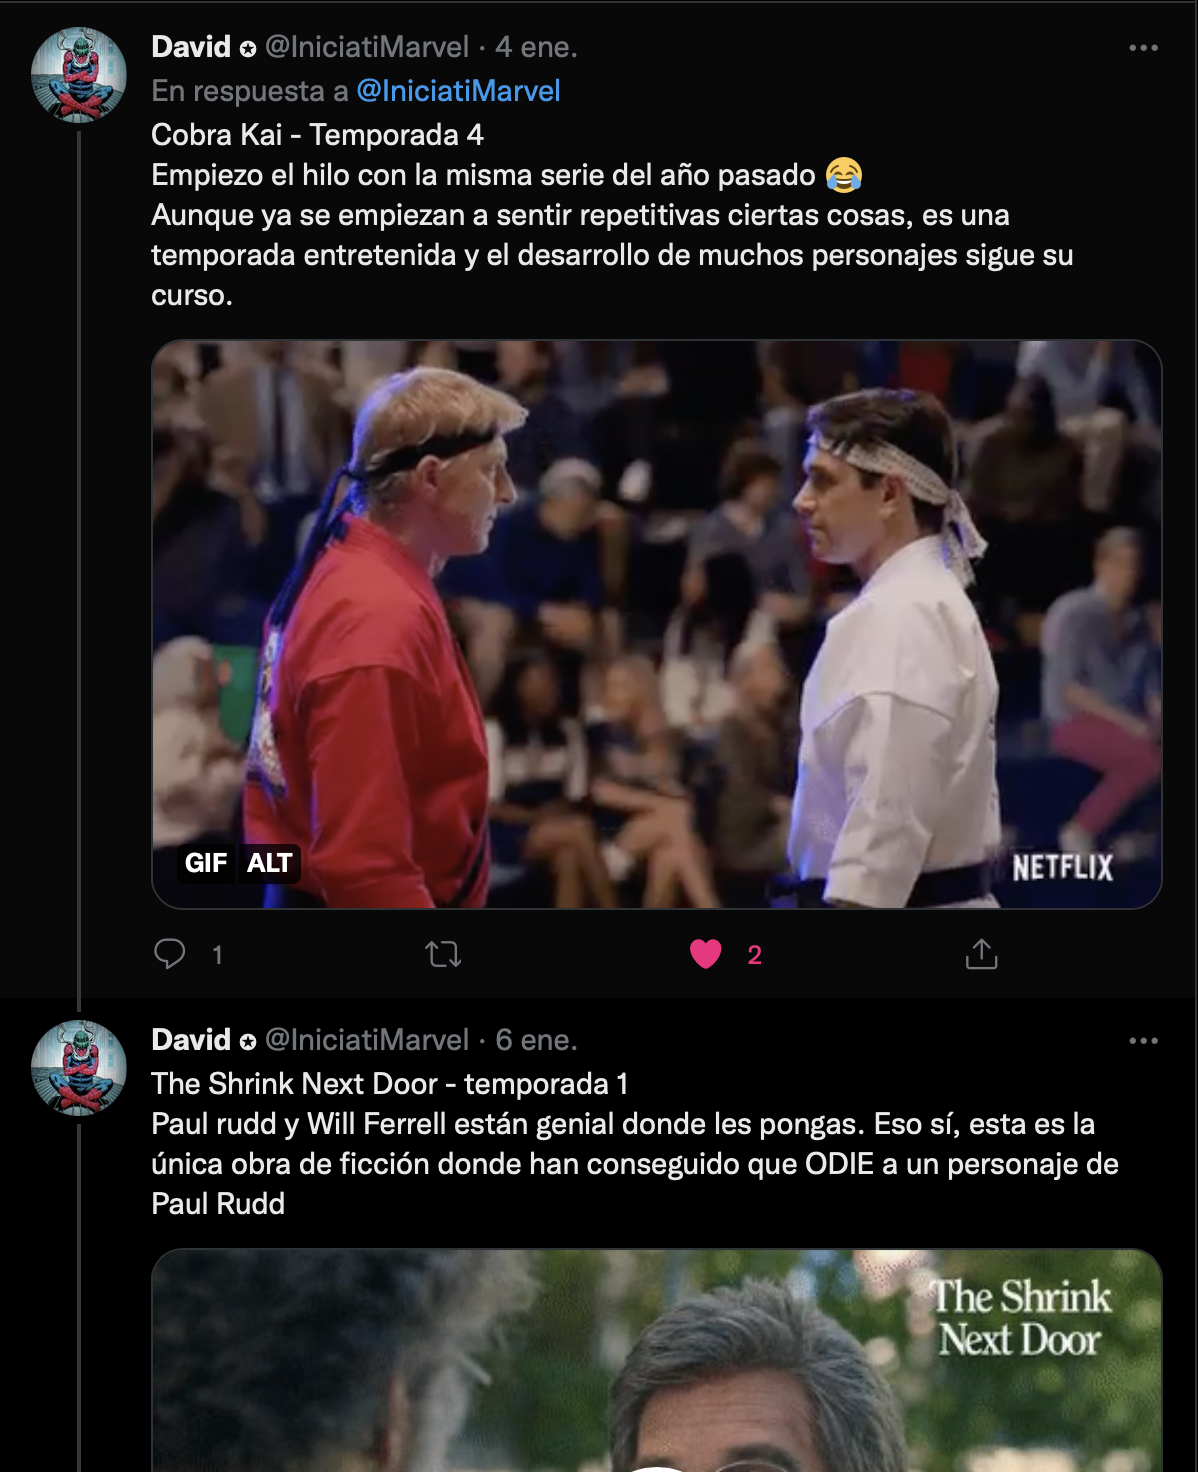
\includegraphics[scale=0.253]{img/twitter-thread-2.png}
	\caption{ @AcolyteJoel y @IniciatiMarvel, usuarios de Twitter, comentando su opinión sobre las series que han visto. }
    \label{fig:twitter_threads}
\end{figure}

\section{Objetivos}
El objetivo principal de este proyecto es crear una aplicación web en la que los usuarios puedan:
\begin{itemize}
    \item \textbf{Escribir} reseñas sobre las series que han visto.
    \item \textbf{Seguir} a otros usuarios para conocer su opinión sobre las series que éstos hayan visto.
    \item \textbf{Leer} reseñas de otros usuarios sobre las series que han visto.
\end{itemize}

Otro objetivo del proyecto, es desarrollar una versión móvil de la aplicación, para que los usuarios puedan hacer uso de la misma desde sus dispositivos móviles.

	% Estado del arte
	% 	1. Crítica al estado del arte
	% 	2. Propuesta
	\chapter{Estado del arte}
En este capítulo se pretende exponer y analizar las distintas propuestas a la hora de resolver los dos problemas que
trata de resolver el proyecto: ayudar al usuario a encontrar una serie que le interese y actuar como una red social en
la que los usuarios discutan su opinión sobre las distintas series que han visto. De esta forma, estudiando los puntos
fuertes y débiles del resto de soluciones, llegaremos a nuestra propia propuesta de valor.\\

\section{Análisis del mercado}
\subsection{IMDB y Rotten Tomatoes}
Existen infinidad de aplicaciones, tanto móvil como web, que tratan de resolver el problema de no saber qué serie o
película elegir. Las más conocidas, y en las que primero fijaremos nuestra mirada, son \href{https://www.imdb.com}
{IMDB} y \href{https://www.rottentomatoes.com}{Rotten Tomatoes}.\\

En ambas, los usuarios puntúan una serie de películas o series y éstas son presentadas en un ranking, de forma que
las más valoradas aparecen en los primeros puestos, indicando que son mejores. Este método, aunque pueda tener
sentido, es ineficiente a la hora de elegir una serie que te guste, ya que aunque una serie esté bien valorada por
el resto de usuarios o por la crítica, no te tiene por qué gustar. Por lo tanto, no resuelven satisfactoriamente
el problema de encontrar una serie interesante para el usuario.\\

También permiten que los usuarios escriban un comentario que sirva de reseña para lo demás. Pero estos comentarios
pasan bastante desapercibidos, ya que para leerlos tienes que abrir la información de la serie y navegar hasta las
últimas secciones en donde se encuentran. Además, la interfaz no es agradable y te redirige a aplicaciones externas de
reseñas, por lo que no funciona eficientemente como una red social.

\begin{figure}[H]
    \centering	
    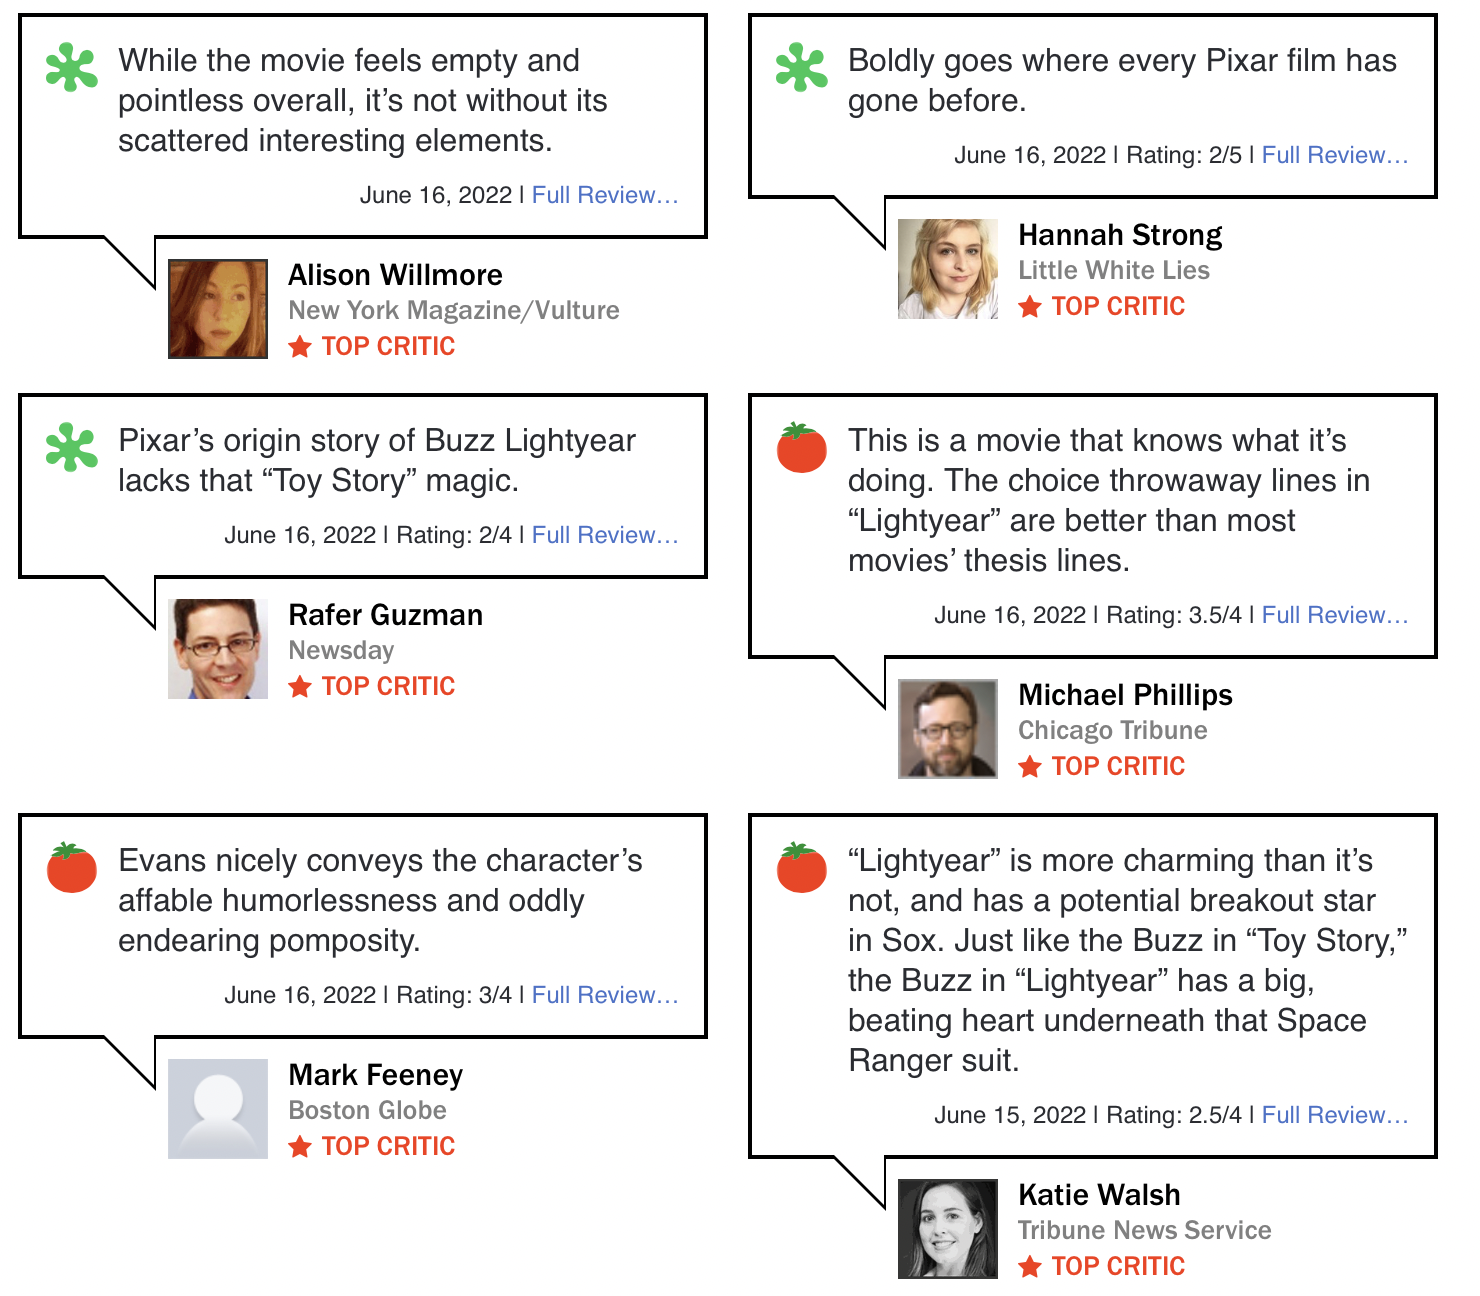
\includegraphics[scale=0.25]{img/rotten-tomatoes-comments.png}
    \caption{ Interfaz de comentarios de Rotten Tomatoes }\label{fig:rotten_tomatoes}
\end{figure}

\subsection{Letterboxd}
Por su parte, \href{https://letterboxd.com}{Letterboxd} sí que se siente más como una red social centrada en las
reseñas. Dándoles más importancia en el feed principal de la aplicación, en el que aparecen tanto las reseñas populares
entre demás usuarios y las de los usuarios que tú sigues. También permite comentar las reseñas de los demás usuarios.
Además, ofrece información sobre las distintas películas de la base de datos. De esta forma, Letterboxd se ofrece como
una solución mucho más acertada a los problemas planteados en este proyecto.

\begin{figure}[H]
    \centering	
    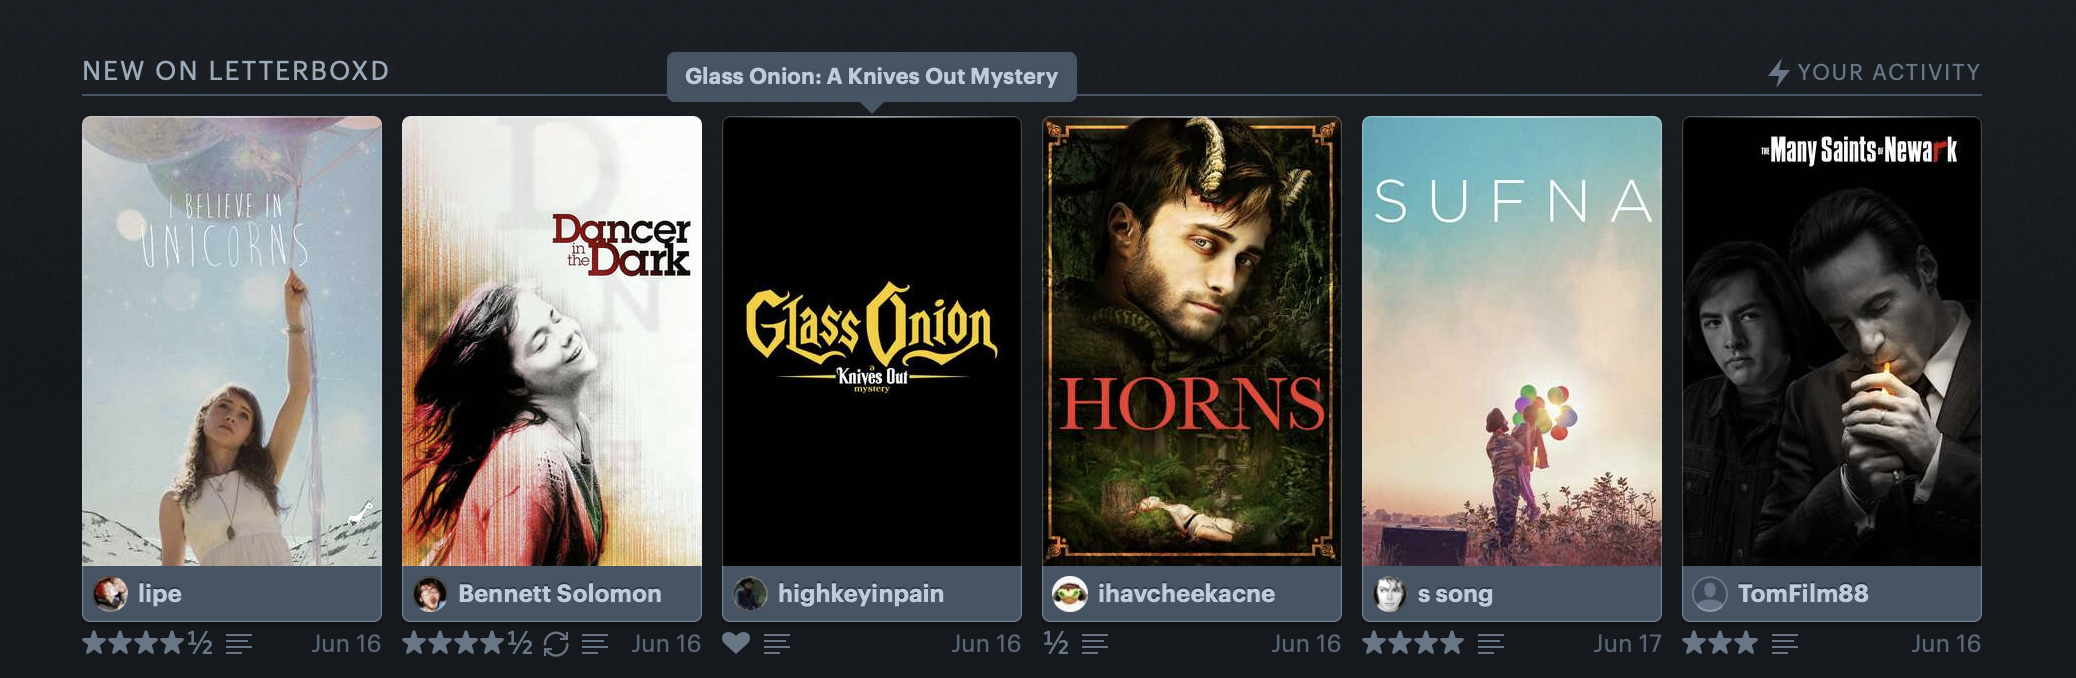
\includegraphics[scale=0.4]{img/letterboxd-feed.png}
    \caption{ Feed de la aplicación Letterboxd }\label{fig:letterboxd}
\end{figure}

Entonces, ¿por qué realizar una nueva aplicación? Los dos inconvenientes de Letterboxd son su interfaz algo desfasada
y que solo permite realizar reseñas de películas, por lo que nuestros usuarios \textit{seriéfilos} son dejados de lado
en esta aplicación.

\section{Mi propuesta ante el estado del arte}
Tras analizar las soluciones existentes y contrastarlas con los \hyperref[sec:objetivo]{objetivos} y requisitos de los
\hyperref[chap:personas]{usuarios} del proyecto, he obtenido una serie de conocimientos que me permitirán desarrollar
una solución que no cometa los mismos fallos que el resto. \\

Para cerrar el capítulo, expondré brevemente los puntos por los que ha de guiarse la solución. 

\begin{itemize}
    \item Feed de la aplicación centrado en las reseñas, mostrando las reseñas de usuarios populares y de los usuarios
    que sigues.
    \item Permitir comentar sobre las reseñas de otros usuarios, dando mayor sensación de red social.
    \item Dar cobertura a las series en lugar de a las películas.
    \item Interfaz moderna, agradable a la vista y user-friendly.
\end{itemize}

	
	\chapter{Metodología}\label{chap:metodología}
Para empezar a desarrollar la solución al problema, primero hay que establecer la metodología de su desarrollo y
control de calidad.

\section{Principios para el desarrollo}
Para el desarrollo del proyecto, tenía claro que quería utilizar una metodología basada en los principios del
manifiesto ágil\cite{agile}. Éstas se basan en la aportación frecuente de código que tenga valor para el usuario, lo
permite una rápida retroalimentación por parte de los usuarios y hace que el desarrollo sea muy flexible a posibles
cambios en alguna funcionalidad.\\

Las metodologías de desarrollo basadas en dichos principios más utilizadas son Kanban\cite{kanban} y Scrum\cite{scrum}.
Scrum se basa en ciclos cortos de trabajo en los que cada periodo determinado de tiempo lo más corto posible,
usualmente una o dos semanas, el cliente recibe un avance en el código de acuerdo a una previa planificación de los
desarrolladores. Esta metodología es perfecta para empresas, ya que facilita las reuniones con los clientes al fijar la
duración de los ciclos y les permite saber de antemano en qué están trabajando los desarrolladores en cada ciclo,
sabiendo qué se van a encontrar en la siguiente versión del proyecto y permitiéndoles influir en la planificación de
los ciclos en base a las funcionalidades más prioritarias para ellos.\\

Aunque la metodología scrum resulta muy útil cuando hay un cliente al que satisfacer con tiempos de entrega y para
planificar de acuerdo a unas prioridades las tareas a realizar por un equipo de trabajo. En este proyecto en el que no
hay un cliente, por lo que es flexible en cuanto a tiempos de entrega, y solo hay un desarrollador, no le estaría
sacando el máximo partido a la metodología scrum.\\

Por tanto, para el desarrollo del proyecto, se optado por seguir la metodología Kanban. Que permite un seguimiento
visual del proyecto en el que se puede ver en todo momento qué tareas se deben hacer, cuáles están en desarrollo y
cuáles se han terminado ya. Apoyándonos en una tabla Kanban los usuarios pueden ver en todo momento el estado del
proyecto y las nuevas funcionalidades en las que se está trabajando.

\begin{figure}[H]
	\centering	
	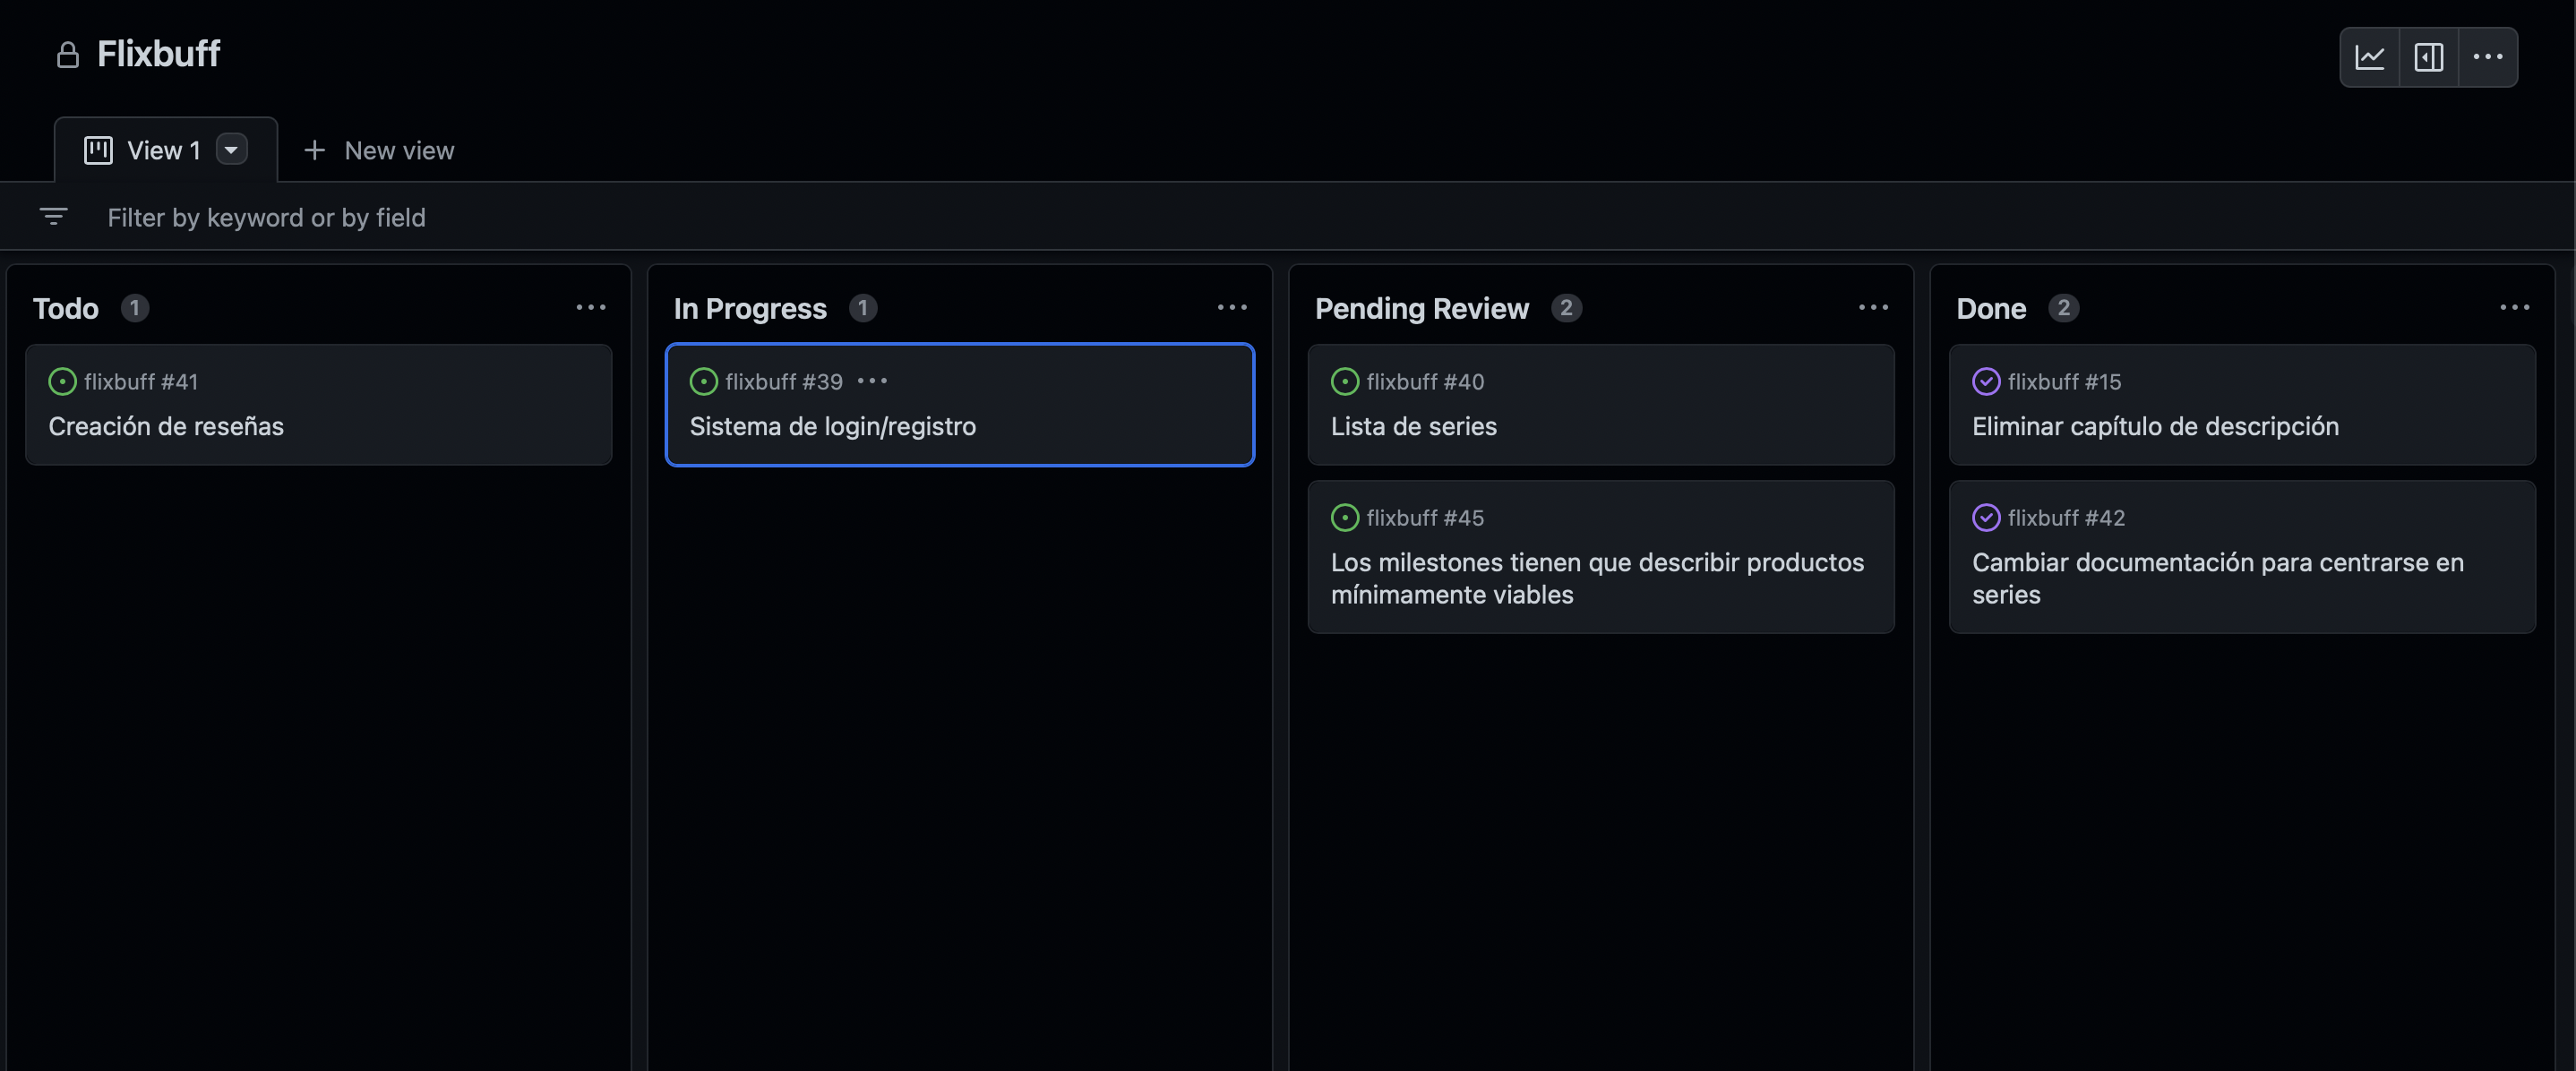
\includegraphics[scale=0.25]{img/kanban.png}
	\caption{\href{https://github.com/users/Torchu/projects/2}{Kanban} del proyecto}\label{fig:kanban_table}
\end{figure}

\subsection{Seguimiento del desarrollo}
Para la transparencia y visualización del proyecto a lo largo de sus diferentes fases, debemos de poder acceder a
estados anteriores en su desarrollo. Para ello, utilizaremos Git, un sistema de control de versiones, en el que
fácilmente podemos ver versiones anteriores del proyecto e incluso volver a ellas revirtiendo algunos cambios,
aumentando la adaptabilidad del proyecto a cambios en los requerimientos de los usuarios.\\

Para alojar el código y registrar las tareas a realizar se ha optado por GitHub, ya que con una cuenta de estudiante
nos da acceso a la creación de tableros Kanban, como el mostrado anteriormente, para la organización de las tareas y a
la integración continua, de la que hablaremos más adelante, a través de las GitHub Actions.\\

De esta forma, los \textit{stakeholders}, o personas interesadas en el desarrollo del proyecto, podrán ver en todo
momento en qué fase del desarrollo se encuentra el mismo, y en qué estado está cada una de sus funcionalidades.

\subsection{Épicas}
Las épicas son grandes grupos de funcionalidad, que sirven para desglosar y atacar el problema. No son una solución al
mismo, pero el conjunto de todas ellas sí que contribuye a la solución.\\

En \textit{GitHub} se reflejan como \href{https://github.com/Torchu/flixbuff/milestones}{\textit{milestones}} del
proyecto. En este caso, son la metodología e infraestructura básica, el sistema de reseñas y el sistema de seguidores.

\begin{figure}[H]
	\centering	
	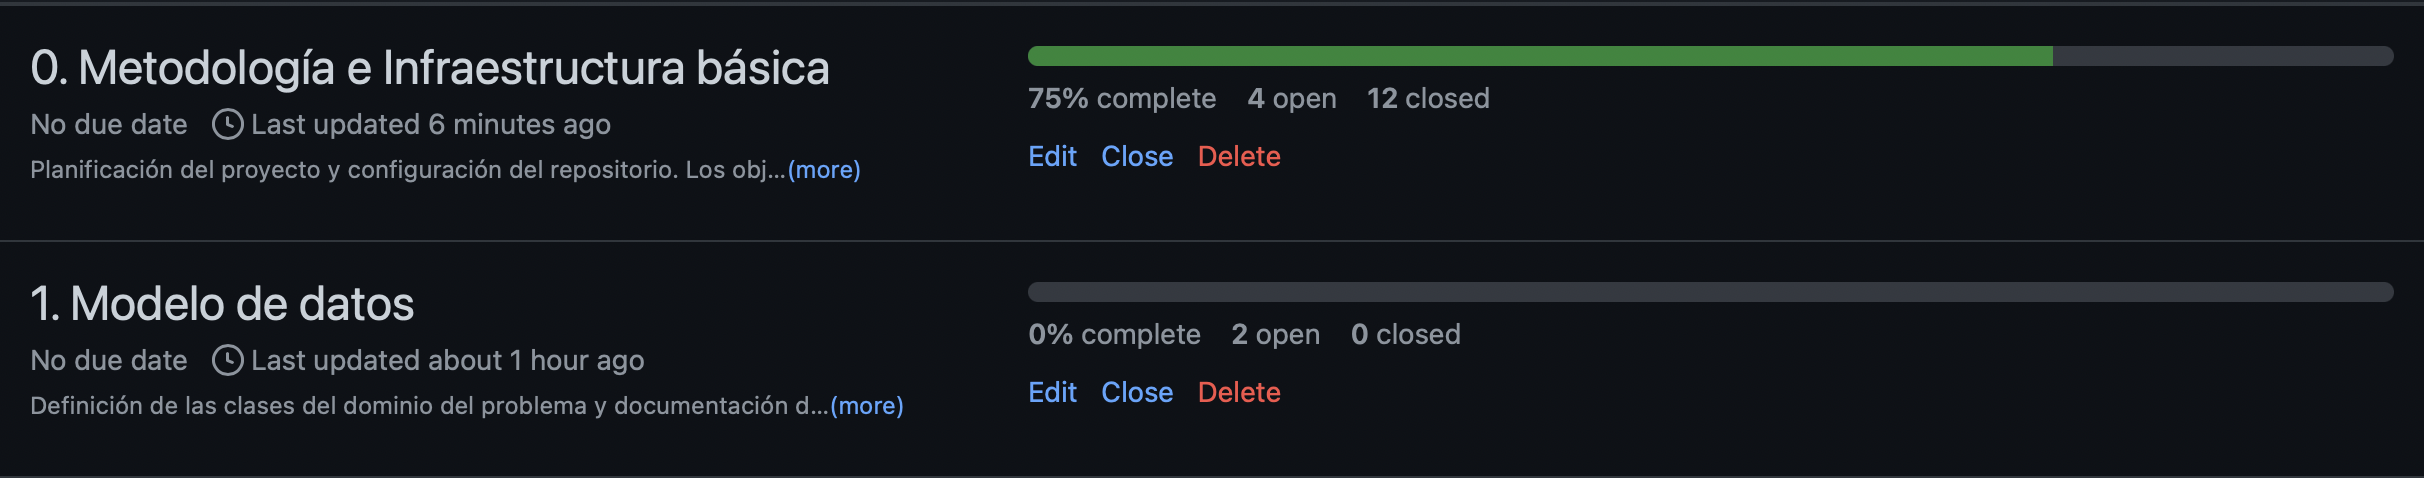
\includegraphics[scale=0.3]{img/milestones.png}
	\caption{\href{https://github.com/Torchu/flixbuff/milestones}{Milestones} del proyecto}\label{fig:github_milestones}
\end{figure}

\subsection{Historias de usuario}
Las épicas a su vez están formadas por historias de usuario. Una historia de usuario es una funcionalidad que el usuario
espera en la solución del problema. Es decir, un requerimiento del usuario.

\begin{figure}[H]
	\centering	
	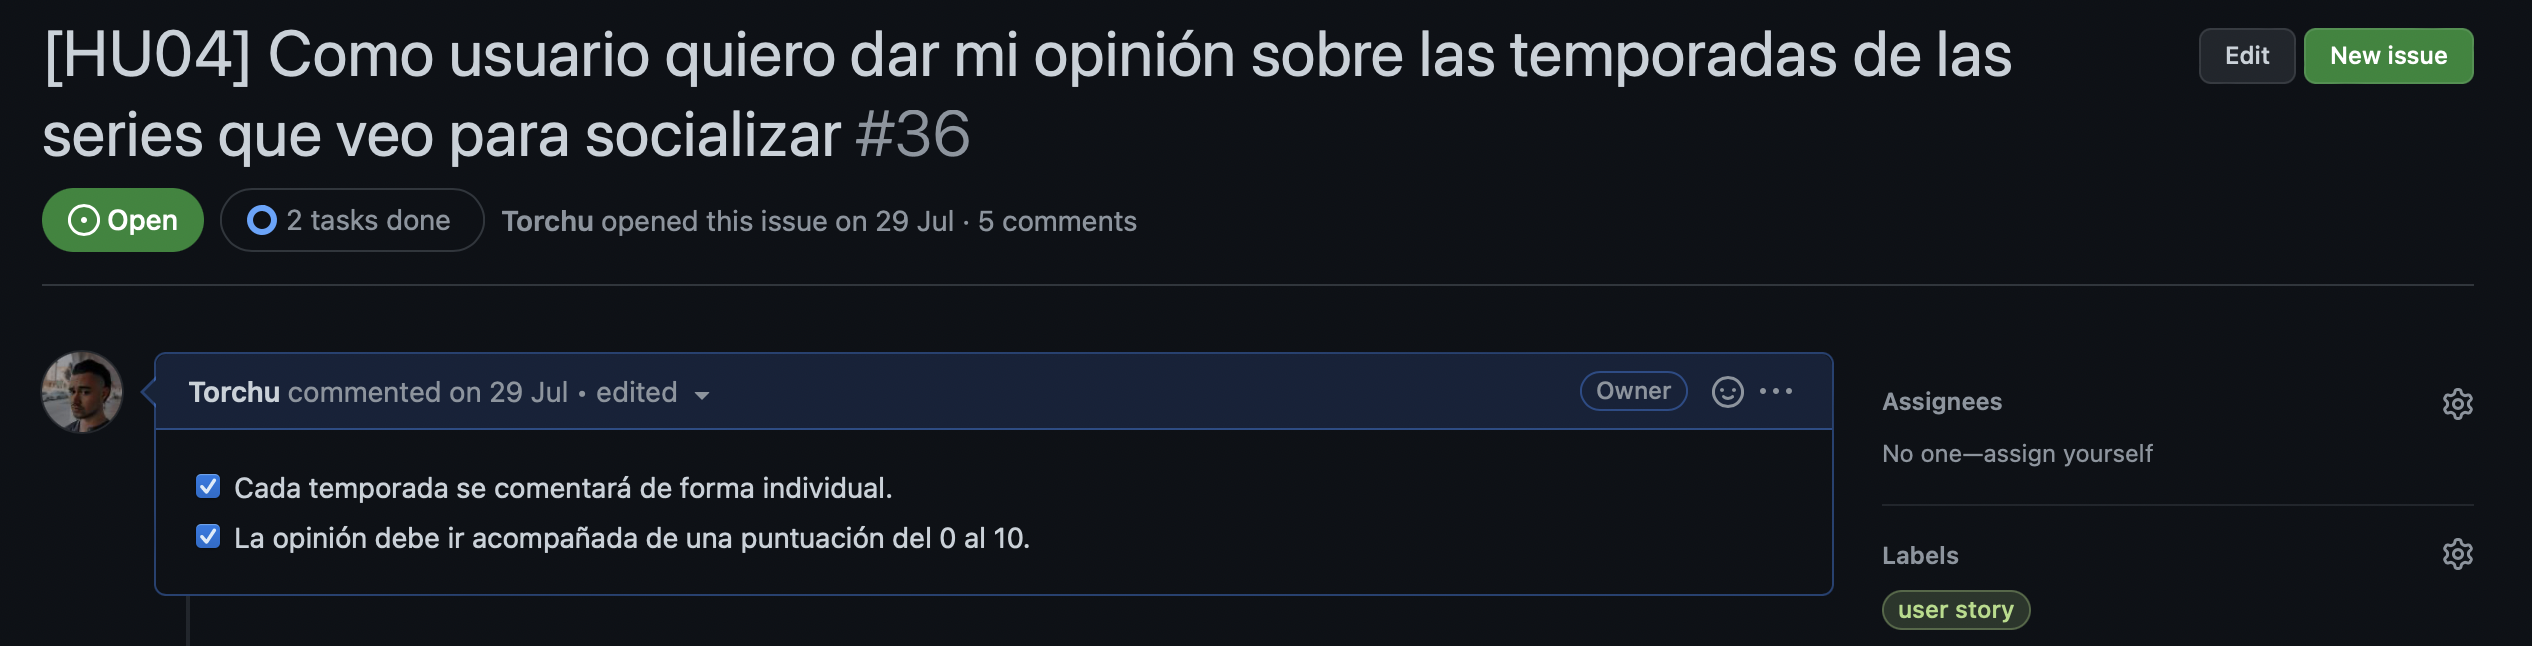
\includegraphics[scale=0.3]{img/user-story.png}
	\caption{Ejemplo de historia de usuario del proyecto}\label{fig:user_story}
\end{figure}

Como en este proyecto no tenemos unos usuarios que nos pidan los requisitos, se ha realizado un análisis de
\textit{Personas}\cite{personas}. Estas personas representan los perfiles de distintos usuarios de la aplicación y
serán ellos quienes nos ayuden con el diseño del producto general, protagonizando las historias de usuario. Ver
\autoref{chap:personas}.

\subsection{Issues}
Las \textit{issues} son problemas que se han detectado en el proyecto y que deben ser resueltos. Los issues se cerrarán
con un \textit{pull request} que incluya una solucione el problema y un test que compruebe que no volverá a pasar.

\begin{figure}[H]
	\centering	
	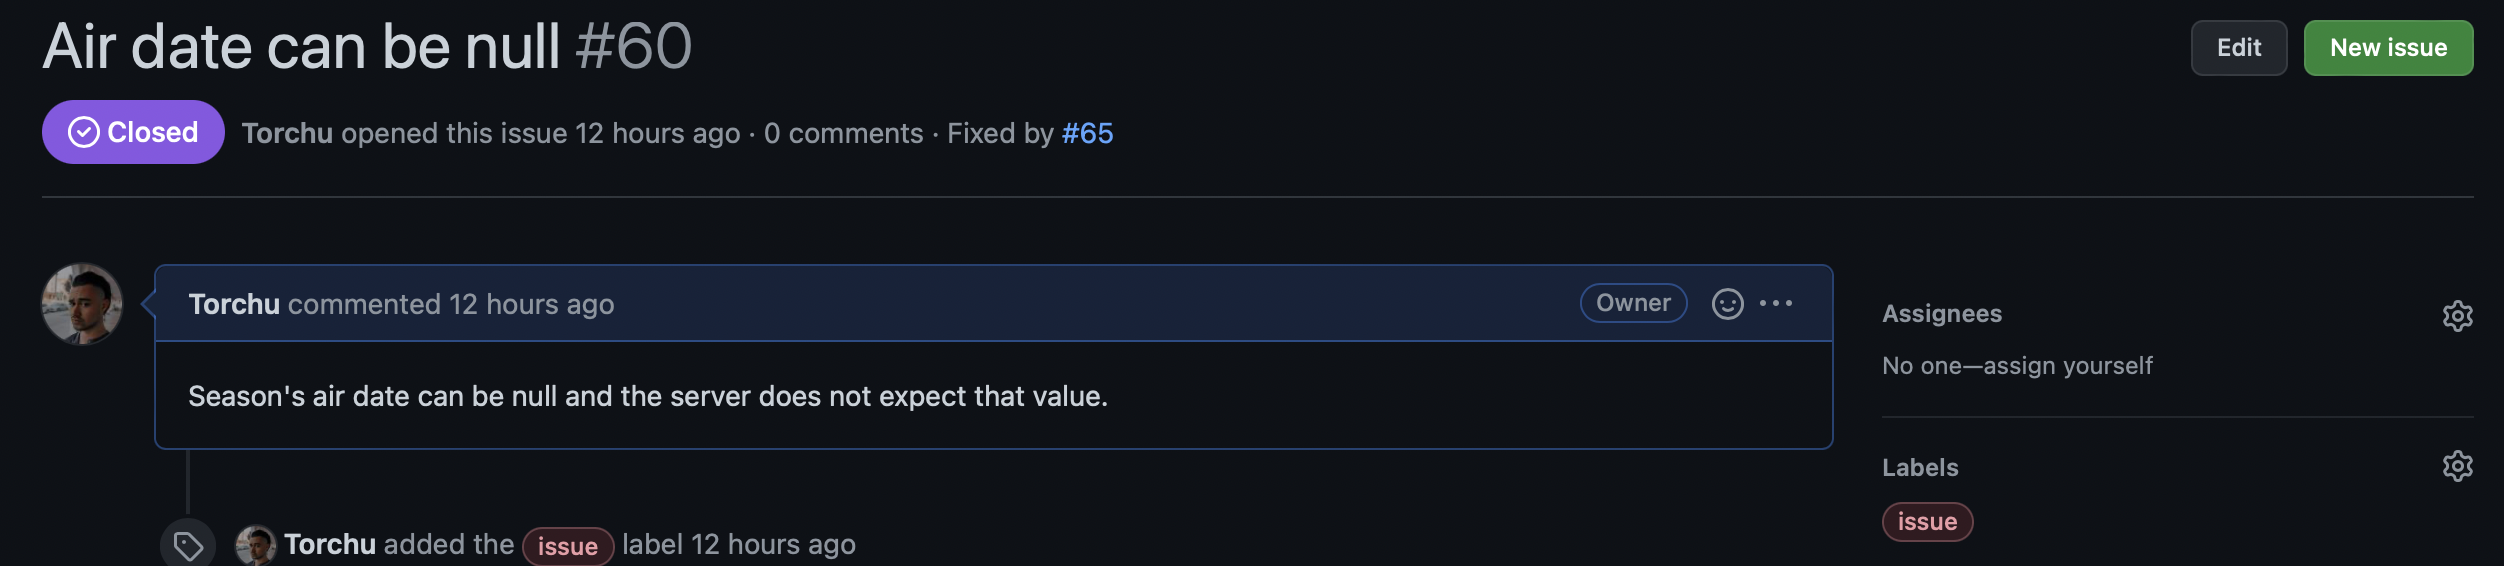
\includegraphics[scale=0.285]{img/issue.png}
	\caption{Ejemplo de issue del proyecto}\label{fig:issue}
\end{figure}

\subsection{Tareas del desarrollador}
Representan pequeñas tareas que facilitan la vida del desarrollador, pero que no representan una funcionalidad como tal.
Por ejemplo, la configuración de la integración continua o tareas para mejorar la organización del código.

\begin{figure}[H]
	\centering	
	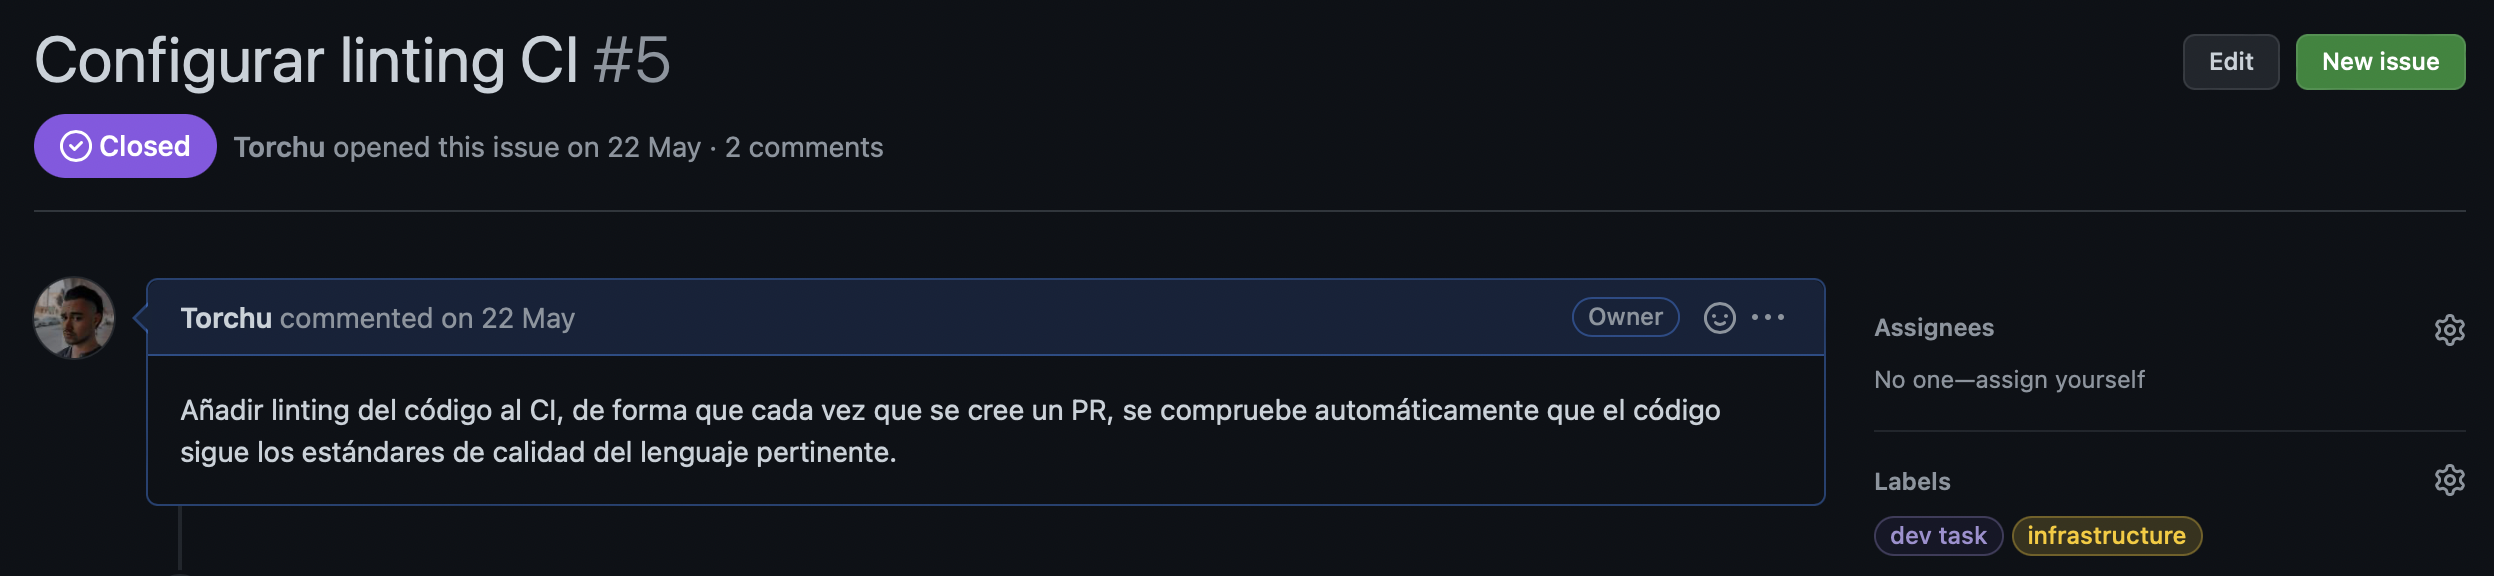
\includegraphics[scale=0.285]{img/dev-task.png}
	\caption{Ejemplo de tarea para el desarrollador del proyecto}\label{fig:dev-task}
\end{figure}

\section{Control de calidad}\label{sec:control_de_calidad}
Para asegurar la calidad del proyecto se ha seguido desde el comienzo del proyecto el desarrollo guiado por pruebas o
TDD\cite{TDD}.\\

Basándonos en esta metodología de desarrollo, trasladaremos los requisitos a una serie de pruebas dentro de nuestro
código, que se crearán antes del desarrollo de las funcionalidades. De esta forma, se convierten tanto en una
documentación fiable, que comprueba que el código desarrollado cumple los requisitos, como en una herramienta de
seguridad, que nos asegura que el código permanezca siempre correcto cada vez que se produzca algún cambio en el
mismo.

\begin{figure}[H]
	\centering	
	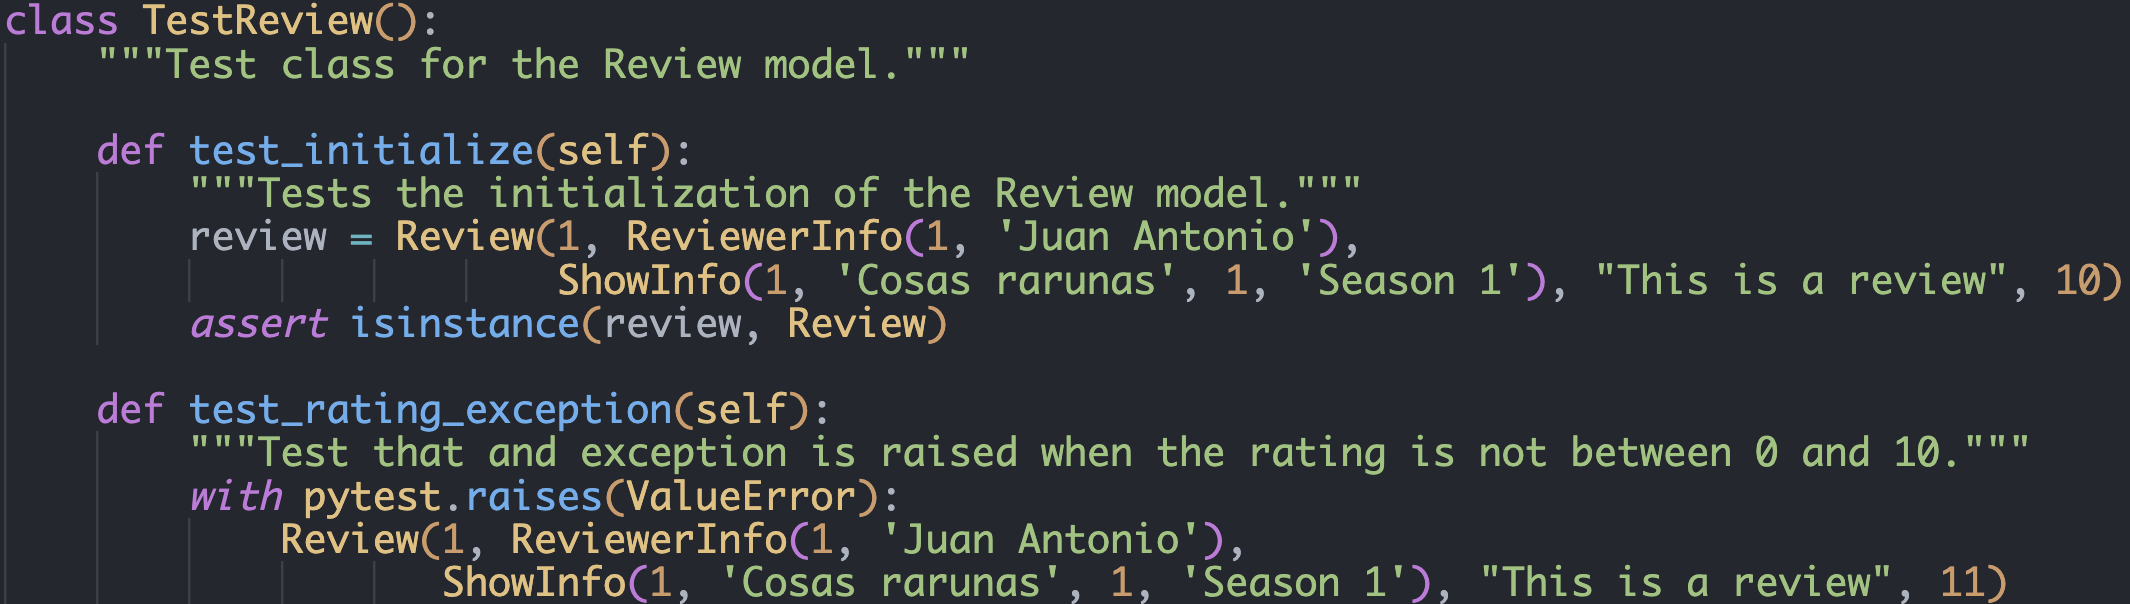
\includegraphics[scale=0.325]{img/pytest.png}
	\caption{Tests de código}\label{fig:tests}
\end{figure}

Además del desarrollo guiado por pruebas, se han configurado una serie de \textit{linters}. Unas herramientas que
comprueban que la sintaxis del código es correcta y cumplimenta la guía de estilo del lenguaje de programación en el
que está desarrollado, dando al desarrollador retroalimentación automática, reduciendo los costes de los posibles
cambios futuros, tal y como establece el desarrollo ágil.\\

Finalmente, se ha incluido un \textit{script} que comprueba la ortografía de toda la documentación del proyecto.
Sirviendo como un \textit{linter} para la documentación, como se recoge en la siguiente
\href{https://github.com/Torchu/flixbuff/issues/4}{historia de usuario}.

\subsection{Integración continua}
La integración continua es una metodología de trabajo que se basa en realizar integraciones frecuentes del código y
asegurarnos que superen los distintos controles de calidad, necesaria para respetar el noveno principio del manifiesto.
ágil:

\begin{quote}
    Continuous attention to technical excellence and good design enhances agility.
\end{quote}

Estos controles de calidad se comprueban mediante las \textit{pipelines}, o acciones que se ejecutan al subir código
al repositorio de GitHub. En nuestro caso incluiremos todo lo mencionado en el apartado
\hyperref[sec:control_de_calidad]{anterior}: pruebas de funcionalidad, \textit{linters} y revisión ortográfica.\\

Para este proyecto,se han configurado las \textit{pipelines} con la herramienta GitHub Actions. Se ha escogido esta
herramienta, ya que es propia de GitHub, la plataforma en la que se aloja el código del proyecto, por lo que no
necesitaremos configurar una herramienta externa. Además, es muy fácil de configurar. Simplemente incluyendo un fichero
yaml en el directorio \textit{.github/workflows/} la propia plataforma ya es capaz de reconocer y ejecutar las
\textit{pipelines} que se han configurado.\\

Se ha optado por una única herramienta para las \textit{pipelines}, ya que al tener solo una reduce el mantenimiento de
la infraestructura y aumenta la velocidad de los despliegues. Quizá en otros proyectos sea interesante mantener dos
herramientas, ya que si hay algún problema en una, no se detiene la integración de código. En este caso, al ser la
herramienta propia de la plataforma en la que se aloja el código, si se cae la plataforma, tampoco podríamos integrar
nuevo código al proyecto, por lo que no es necesaria una segunda herramienta.

\begin{figure}[H]
	\centering	
	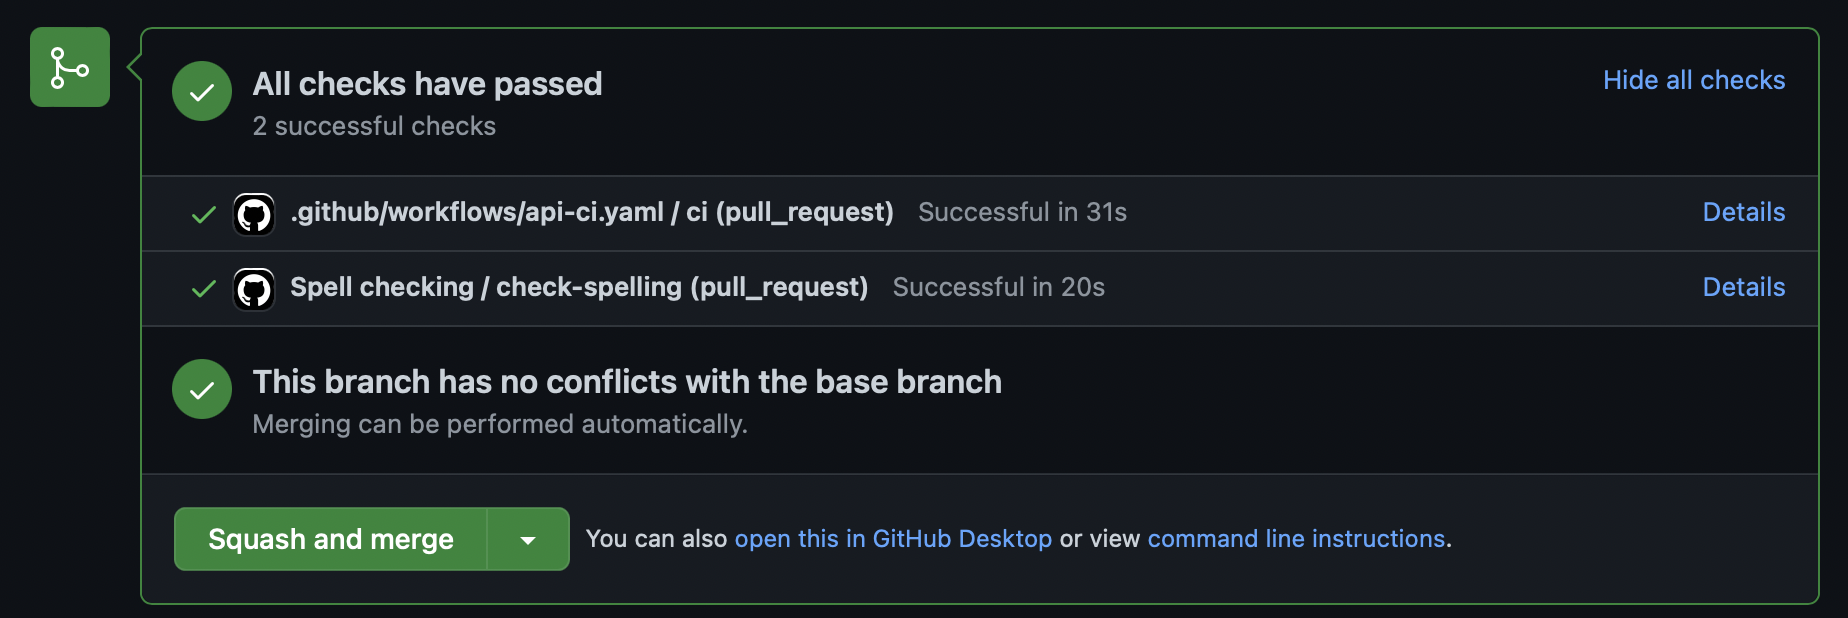
\includegraphics[scale=0.4]{img/pipeline.png}
	\caption{Pipeline de aprobado de un PR}\label{fig:pipeline_succeded}
\end{figure}


	% Análisis del problema
	% 1. Análisis de requisitos
	% 2. Análisis de las soluciones
	% 3. Solucion propuesta
	% 4. Análisis de seguridad
	\chapter{Análisis de los costes}
En esta sección se analizarán y desglosarán los costes de llevar a cabo el proyecto\\

\begin{table}[H]
    \centering
    \begin{center}
        \begin{tabular}{| p{0.3\linewidth} | p{0.2\linewidth} | p{0.35\linewidth}|}
            \hline
            \rowcolor[HTML]{ECF4FF} 
            \textbf{Concepto} & \textbf{Coste} & \textbf{Comentarios}\\ \hline
            \textbf{MacBook Pro M1 2021} & 150 €/año & La cantidad de amortización aplicable es del 26\% a 10 años. Con
            coste de compra: 1500€\\
            \textbf{Recursos software} & 0 € & No se ha utilizado ninguna librería de pago para la realización del
            proyecto.\\
            \textbf{Recursos para el despliegue } & 2 X (Desde 0 a 100€/mes) & Dependiendo de la \textit{tier} y los
            \textit{dynos} utilizados. Se multiplica por dos al ser dos aplicaciones desplegadas. Puede consultarse en
            mayor detalle en la sección de \hyperref[sec:costes-despliegue]{costes del despliegue}.\\
            \textbf{Recursos para la base de datos} & Desde 0 a €/mes & Dependiendo de la \textit{tier}.\\
            \hline
        \end{tabular}
        \caption{Presupuesto del proyecto.}
    \end{center}
\end{table}


	% Desarrollo bajo sprints: 
	% 	1. Permitir registros y login de usuarios
	% 	2. Desarrollo del sistema de incidencias
	% 	3. Desarrollo del sistema de denuncias administrativas y accidentes
	% 	4. Desarrollo del sistema de croquis
	%   5. Instalación de la aplicación de manera automática
	\chapter{Implementación}\label{chap:implementación}
Para la implementación de la solución utilizaremos una arquitectura cliente-servidor\cite{client-server}, la cual nos
permite tener los datos centralizados en una aplicación servidor. La aplicación cliente realizará peticiones al
servidor, para que este le provea de los datos que necesite en cada momento.

\section{Servidor}
En el lado del servidor o \textit{back-end} se encuentra la mayor parte de la lógica de la aplicación, dedicándose el
lado del cliente a simplemente mostrarla en una interfaz cómoda para el usuario.\\

Se ha implementado un servidor que provee a los clientes de un listado de series y sus temporadas, así como de la
posibilidad de crear reseñas de las mismas o obtener las reseñas de otros usuarios.

\subsection{Lenguaje de programación}
El lenguaje de programación seleccionado para el servidor es \textit{Python}\cite{python}, ya que es un lenguaje de
programación que nos provee de una buena experiencia de desarrollo al ser un lenguaje menos estricto y cuenta con muchas
librerías útiles y una enorme comunidad a sus espaldas.\\

Uno de sus puntos débiles, es que al ser un lenguaje no tipado, es más propenso a errores de sintaxis, pero desde la
versión 3.5, cuenta con una forma de tipar el código, de forma que, aunque el intérprete de \textit{Python} no detecte
este tipado, puede ser utilizado por herramientas de los \textit{IDEs} y \textit{linters} para la detección precoz
errores.\\

Otro de los motivos que me han llevado a decantarme por este lenguaje son sus librerías científicas y de procesamiento
de datos. Con ellas, en un futuro podríamos incluir en la aplicación alguna herramienta para obtener estadísticas y
realizar predicciones sobre nuestros datos. Algo muy útil para un cliente que quiera usar los datos de la aplicación
para saber qué tipo de series interesan a cierto tipo de público, por ejemplo.\\

Como gestor de paquetes y dependencias, utilizo \textit{poetry}\cite{poetry}, que nos permite gestionar las dependencias
del proyecto de forma muy sencilla y similar a \textit{NPM}\cite{npm}.

\subsection{Framework}
El framework utilizado para el servidor es \textit{Flask}\cite{flask}, un framework de Python que nos permite una 
\textit{REST API}\cite{rest} minimalista, flexible y fácil de usar.

\subsection{Operaciones}
Recopilación y breve descripción de las peticiones que atiende el servidor.

\subsubsection{Autenticación}
Los usuarios podrán loguearse con su cuenta, lo que generará un token de acceso que deberá ser enviado en las cabeceras
del resto de peticiones, para identificar qué usuario está realizando la petición, lo que en algunas de las operaciones
será obligatorio.\\

Para asegurarnos que el usuario está logueado, utilizamos un \textit{decorador} de la librería
\textit{Flask-JWT-Extended}\cite{jwt} que comprueba que el token enviado en las cabeceras de la petición es válido. Si
no lo es, se devuelve un error 401, o de desautorización.

\subsubsection{Series}
El servidor provee de una lista de series o de los detalles de una serie en particular o alguna de sus temporadas a
través de su identificador. Sin embargo, la base de datos no incluye la información de estas series, si no que se
obtienen a través de una API externa.\\

La API utilizada es \href{https://www.themoviedb.org}{\textit{TheMovieDB}}, una API abierta que provee de datos sobre
series y películas. En este caso, haremos uso de las series. Gracias al diseño de nuestra aplicación, podríamos cambiar
de API en cualquier momento, sin que suponga mucho tiempo de desarrollo.\\

Además, también provee de una lista de series ordenadas por popularidad, según los rankings de \textit{TheMovieDB}.

\subsubsection{Usuarios}
Cualquiera podrá listar o crear un usuario, siempre y cuando el email introducido no esté en uso.\\

A través de su ID, se podrán acceder a los datos de dicho usuario u obtener las reseñas que ha realizado.\\

Además, los usuarios identificados podrán seguir o dejar de seguir a otros usuarios y obtener la lista de reseñas hechas
por cualquier de los usuarios que están siguiendo.

\subsubsection{Reseñas}
Los usuarios identificados podrán crear reseñas de las series. Usando el token \textit{JWT} del que hablamos en la
sección anterior, podemos obtener el identificador del usuario que está realizando la petición y añadirlo a los datos de
la reseña.\\ 

Además, cualquier usuario - identificado o no - podrá obtener la lista de reseñas hechas en la aplicación, ordenadas de
más a menos recientes.

\subsection{Test}
Como ya hablamos en la \hyperref[chap:metodología]{metodología}, necesitamos que el código cumpla con unos requisitos
mínimos de calidad a través de \textit{tests}.\\

Para el servidor, se han implementado tests unitarios con la librería \textit{pytest}\cite{pytest}, que comprueban que
los métodos de los modelos de la aplicación funcionan correctamente.

\begin{figure}[H]
\centering	
    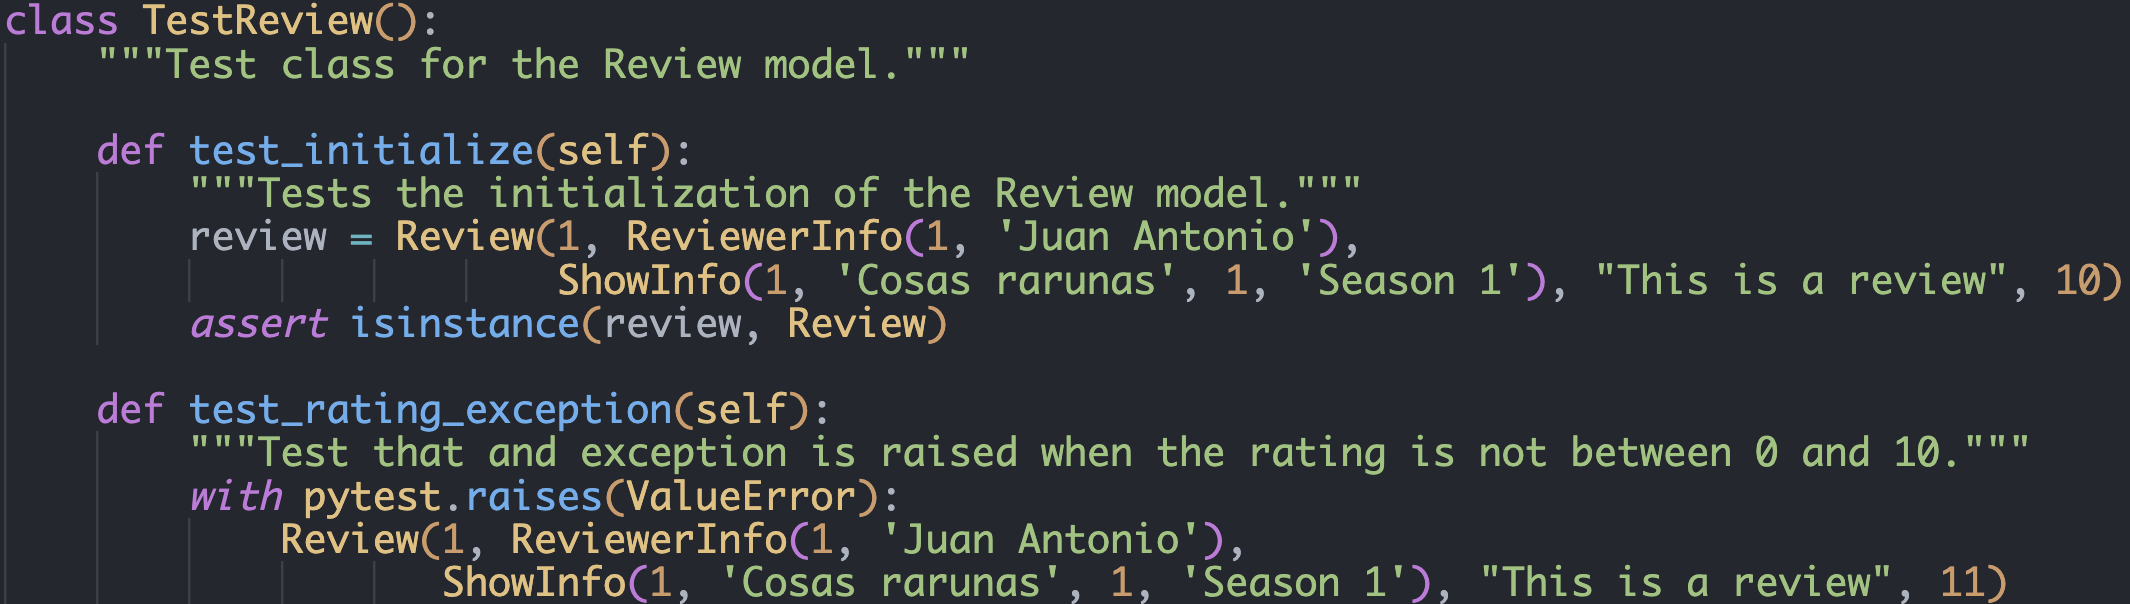
\includegraphics[scale=0.25]{img/pytest.png}
\caption{ Test unitario de la clase Show en Python }\label{fig:pytest}
\end{figure}

\subsection{Base de datos}
El número de reseñas irá en aumento con el tiempo y con el número de usuarios de la aplicación, por lo que necesito una
base de datos que sea fácilmente escalable. Por ello, \textit{MongoDB}\cite{mongodb} es una muy buena opción, gracias a
\textit{MongoAtlas}\cite{mongoatlas}, una herramienta \textit{DataBase as a Service}\cite{dbaas} que nos permite escalar
la base de datos verticalmente, aumentando el poder de procesamiento de nuestro cluster, u horizontalmente, añadiendo
más nodos para compartir la carga.\\

Además, guarda los datos en formato \textit{JSON}\cite{json}, lo que nos permite acceder a ellos de forma muy sencilla y
fácilmente interpretable por cualquier lenguaje de programación moderno.

\subsection{Configuración}
Las variables de configuración se encuentran en los ficheros del directorio \textit{config} y se definen mediante las
variables de entorno, incluyendo opciones por defecto en la mayoría. En el entorno de desarrollo, uso \textit{dotenv}
para cargar las variables de entorno desde un fichero de configuración \textit{.env}.

\begin{figure}[H]
\centering	
    
\includegraphics[scale=0.525]{img/dotenv.png}
\caption{ Fichero de configuración con las variables de entorno del servidor }\label{fig:dotenv}
\end{figure}

Para el entorno de producción, las variables se cargan en \textit{Heroku}\cite{heroku} de forma sencilla, como veremos
en el \hyperref[sec:despliegue]{despliegue}.

\section{Cliente}
El cliente o \textit{back-end} es la parte de la aplicación que se ejecuta en el dispositivo del usuario. En nuestro
caso, la mayor parte de la lógica se encuentra en el lado del servidor y el cliente se encarga de mostrar la información
y dar acceso a las peticiones del servidor de una forma amigable para el usuario.

\subsection{Elección de la tecnología}
Con el paso del tiempo, cada vez más frameworks y librerías se han ido desarrollando para la creación de aplicaciones
cliente, por lo que hay una gran variedad de tecnologías a nuestra disposición.

\subsubsection{Aplicación web vs aplicación móvil}
Es cierto que las aplicaciones móviles están ganando cada vez más popularidad, ya que con la afluencia de dispositivos
inteligentes como teléfonos, tablets, televisores e incluso frigoríficos, es más fácil acceder a la información desde
cualquier parte.\\

No por ello, debemos descartar las aplicaciones web. En este caso, una aplicación web es una solución sólida al
problema, al ser más cómodo para los usuarios escribir sus reseñas con su teclado y ratón, y no con su pantalla
táctil.

\subsubsection{Frameworks}
Los tres grandes framework para aplicaciones web son: \textit{Angular}\cite{angular}, \textit{React}\cite{react} y
\textit{Vue}\cite{vue}.\\

\noindent \textbf{Vue}\\ \\
\indent \textit{Vue} es un framework muy ligero, que se basa en componentes, lo que lo hace muy fácil de aprender y de usar.
Además, permite usar expansiones de terceros para añadir componentes o funcionalidades hechas por la comunidad. Sin
embargo, utiliza \textit{JavaScript}\cite{javascript} como lenguaje de programación, por lo que no es la opción más
deseable frente a los otros dos.\\

\noindent \textbf{React}\\ \\
\indent \textit{React} está basado en \textit{JavaScript} y utiliza \textit{JSX}\cite{jsx} para definir los componentes, aunque
también se puede usar \textit{TypeScript}\cite{typescript}, un lenguaje tipado que se transpila a \textit{JavaScript},
lo que nos permite la detección rápida de errores. Es un framework muy popular y con una gran comunidad detrás, lo que
lo convierte en una buena opción.\\

\noindent \textbf{Angular}\\ \\
\indent Finalmente, el framework que he elegido es \textit{Angular}. Aunque esté perdiendo popularidad, sigue
siendo una gran opción para el desarrollo de aplicaciones web. Trabaja nativamente con \textit{TypeScript}, por lo que
fácilmente podremos disfrutar de las ventajas de un lenguaje tipado.\\

\textit{Angular} es un framework diseñado y mantenido por \textit{Google} que nos ofrece un código bien estructurado
basado en componentes y servicios, que nos permite desarrollar con una arquitectura limpia y mantenible. Además, nos
permite usar \textit{Angular Material}\cite{angularmaterial}, un conjunto de componentes de \textit{Angular} que nos
permite crear interfaces de usuario modernas de forma rápida y sencilla y también cuenta con \textit{Ionic}\cite{ionic},
un framework para crear aplicaciones híbridas para móviles y web si en algún momento decidiésemos dar el salto a las
aplicaciones móviles.

\subsection{Diseño}
En esta sección se detallarán los aspectos de las diferentes vistas de la aplicación. Se ha apostado por un diseño
elegante y minimalista, usando los componentes del ya mencionado \textit{Angular Material}.

\subsubsection{Barra de navegación}
En la parte de arriba de cualquiera de las vistas de la aplicación, se encuentra la barra de navegación.\\

La barra de navegación muestra el título de la aplicación y otras dos pestañas: \textit{Shows} y \textit{Users}.\\

Hacer click en el título redirigirá al usuario a la feed principal de la aplicación, mientras que hacer click en
alguna de las otras dos vistas, le transportará a la lista de series y de usuarios, respectivamente.\\

En la parte derecha de la barra de navegación, nos encontraremos la pestaña de \textit{Log In}, que desplegará la
\hyperref[sec:login-signin]{ventana de registro y logueo}. En caso de ya estar logueado, la pestaña mostrará tu nombre de
usuario y haciendo click, desplegará un menú cuya única opción es el deslogueo.

\begin{figure}[H]
    \centering	
        
\includegraphics[scale=0.25]{img/navbar.png}
    \caption{ Barra de navegación previa al login }\label{fig:navbar}
\end{figure}

\begin{figure}[H]
    \centering	
        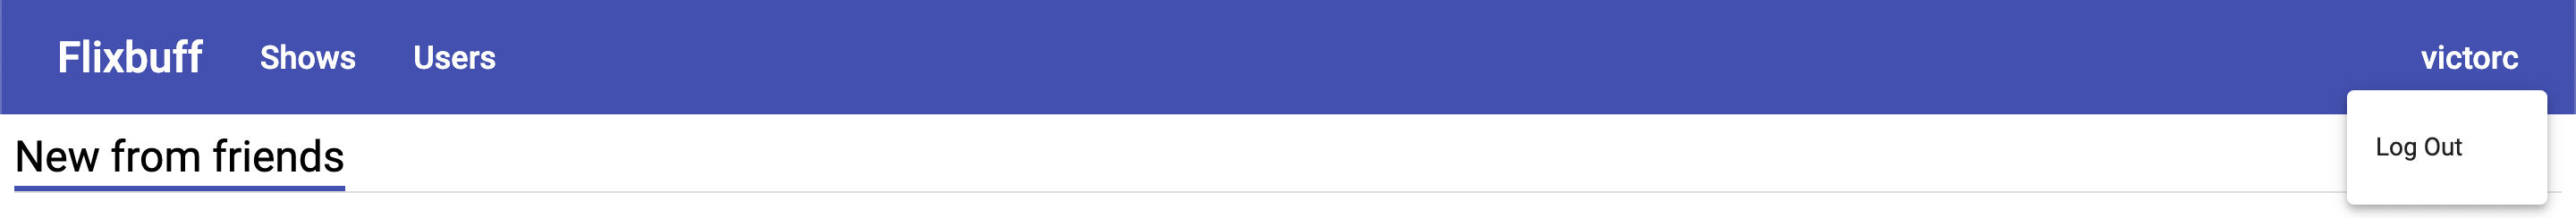
\includegraphics[scale=0.25]{img/logged-navbar.png}
    \caption{ Barra de navegación posterior al login }\label{fig:logged-navbar}
\end{figure}

\subsubsection{Ventana de login/registro}\label{sec:login-signin}
Tras el click en la pestaña de \textit{log in} se despliega esta ventana que se superpone al resto de la aplicación.\\

La ventana está dividida en tres secciones: las pestañas, el formulario y los botones. \\

Las dos pestañas son \textit{Log In} y \textit{Create Account} y modifican el resto de la ventana acorde a la operación
que quieras llevar a cabo, acceso o registro, respectivamente.\\

En la parte baja de la ventana encontramos dos botones, el primero refleja la acción que se intenta llevar a cabo - 
acceso o registro - y no funcionará hasta que los datos del formulario correspondiente sean correctos. El segundo botón
sirve para cancelar la operación y cerrar la ventana.

\begin{figure}[H]
    \centering	
        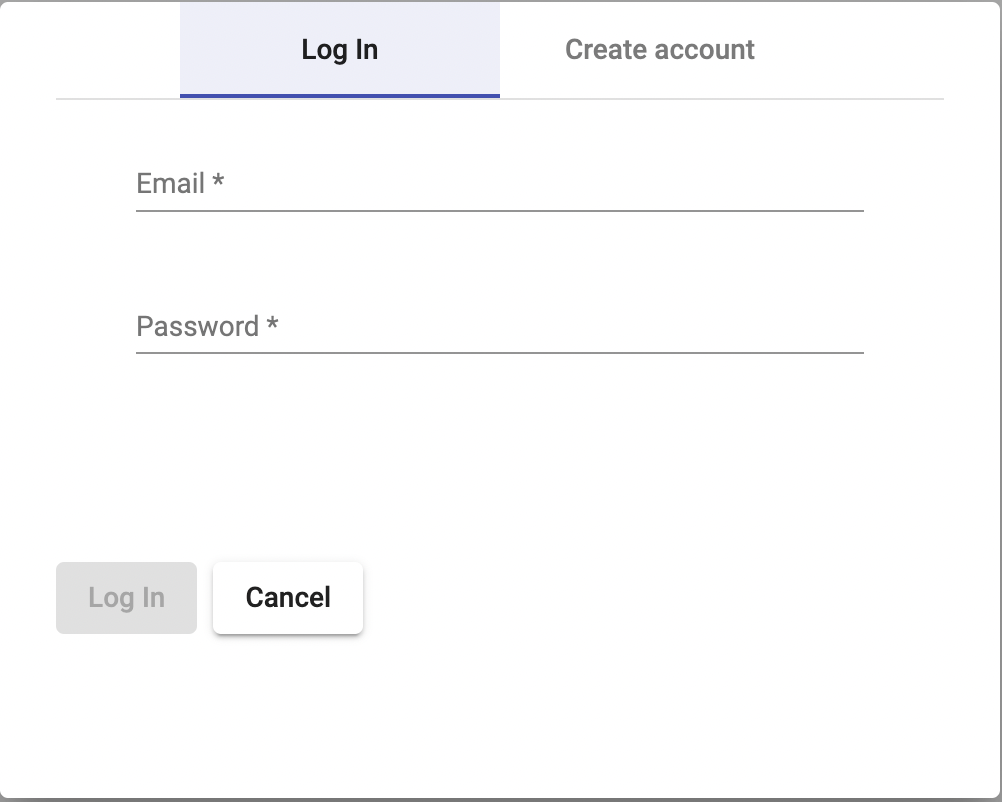
\includegraphics[scale=0.25]{img/login.png}
        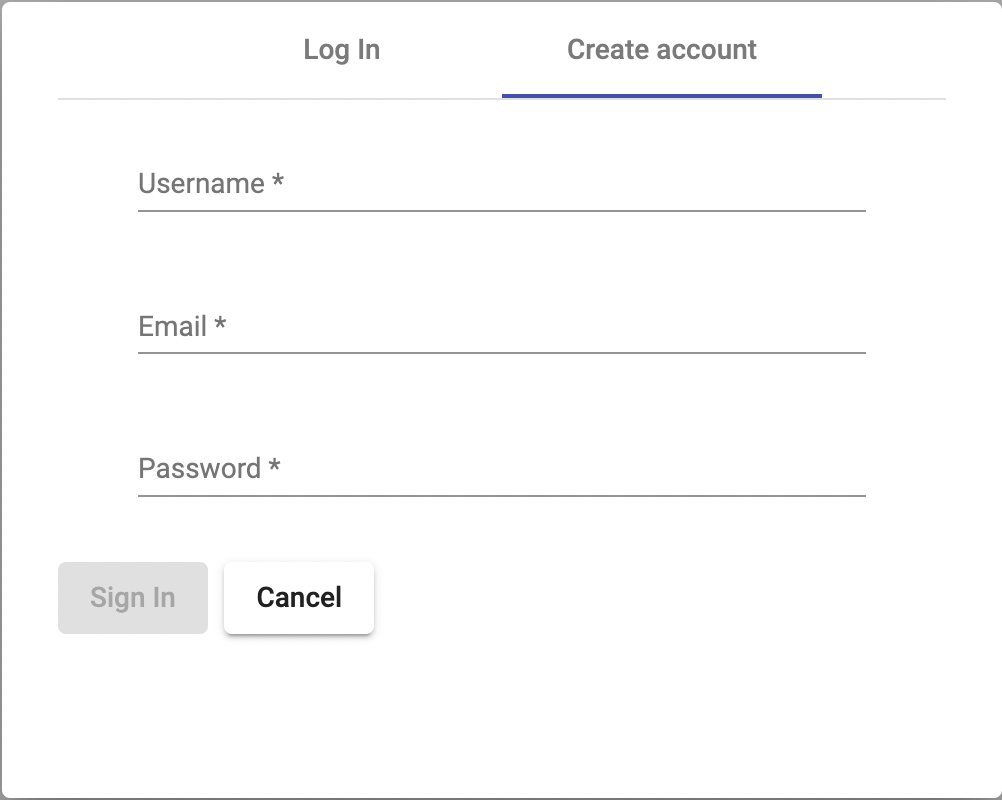
\includegraphics[scale=0.25]{img/signin.png}
    \caption{ Ventana de acceso y registro }\label{fig:login}
\end{figure}

\subsubsection{Feed principal}
El feed principal de la aplicación está compuesto por tres secciones.\\

La primera sección, solo visible a usuarios logueados, muestra las reseñas más recientes de los usuarios a los que
siguen. Las reseñas se muestran en un carrusel de tarjetas y unos botones a los lados que permiten cambiar de página.\\

Estas tarjetas tienen por título el título de la serie y el nombre de la temporada y el nombre del revisor como
subtítulo, acompañados por el texto de la reseña y su puntuación representada por estrellas. Además de el poster de la
temporada en la parte izquierda.

\begin{figure}[H]
    \centering	
        
\includegraphics[scale=0.5]{img/review-card.png}
    \caption{ Tarjeta de reseña }\label{fig:review-card}
\end{figure}

La segunda sección muestra las series más populares del momento, en forma de carrusel de tarjetas, al igual que con las
reseñas. En este caso, las tarjetas incluyen el título de la serie y su fecha, el póster de la obra y un pequeño resumen
de la misma. Hacer click en una serie te llevará a la vista de detalles de la misma.

\begin{figure}[H]
    \centering	
        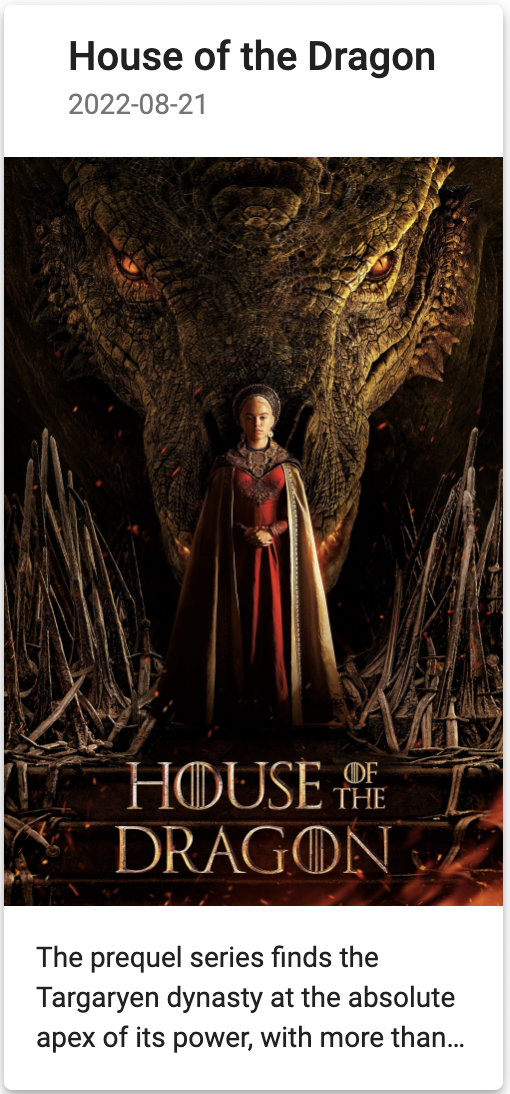
\includegraphics[scale=0.5]{img/show-card.png}
    \caption{ Tarjeta de serie }\label{fig:show-card}
\end{figure}

La tercera sección muestra lo mismo que la primera, pero en este caso muestra la reseñas más recientes de todos los
usuarios de la aplicación. Al hacer click en alguna de ellas, te llevará al perfil del usuario que la escribió, para que
puedas seguirle y ver sus otras reseñas.

\subsubsection{Lista de series}
En la lista de series podemos encontrar una barra de búsqueda en la parte superior de la vista. Al escribir algo en la
barra, automáticamente se buscarán las series que contengan esa cadena en el nombre y se mostrarán en una rejilla de
tarjetas de series como las de la sección anterior.\\

\begin{figure}[H]
    \centering	
        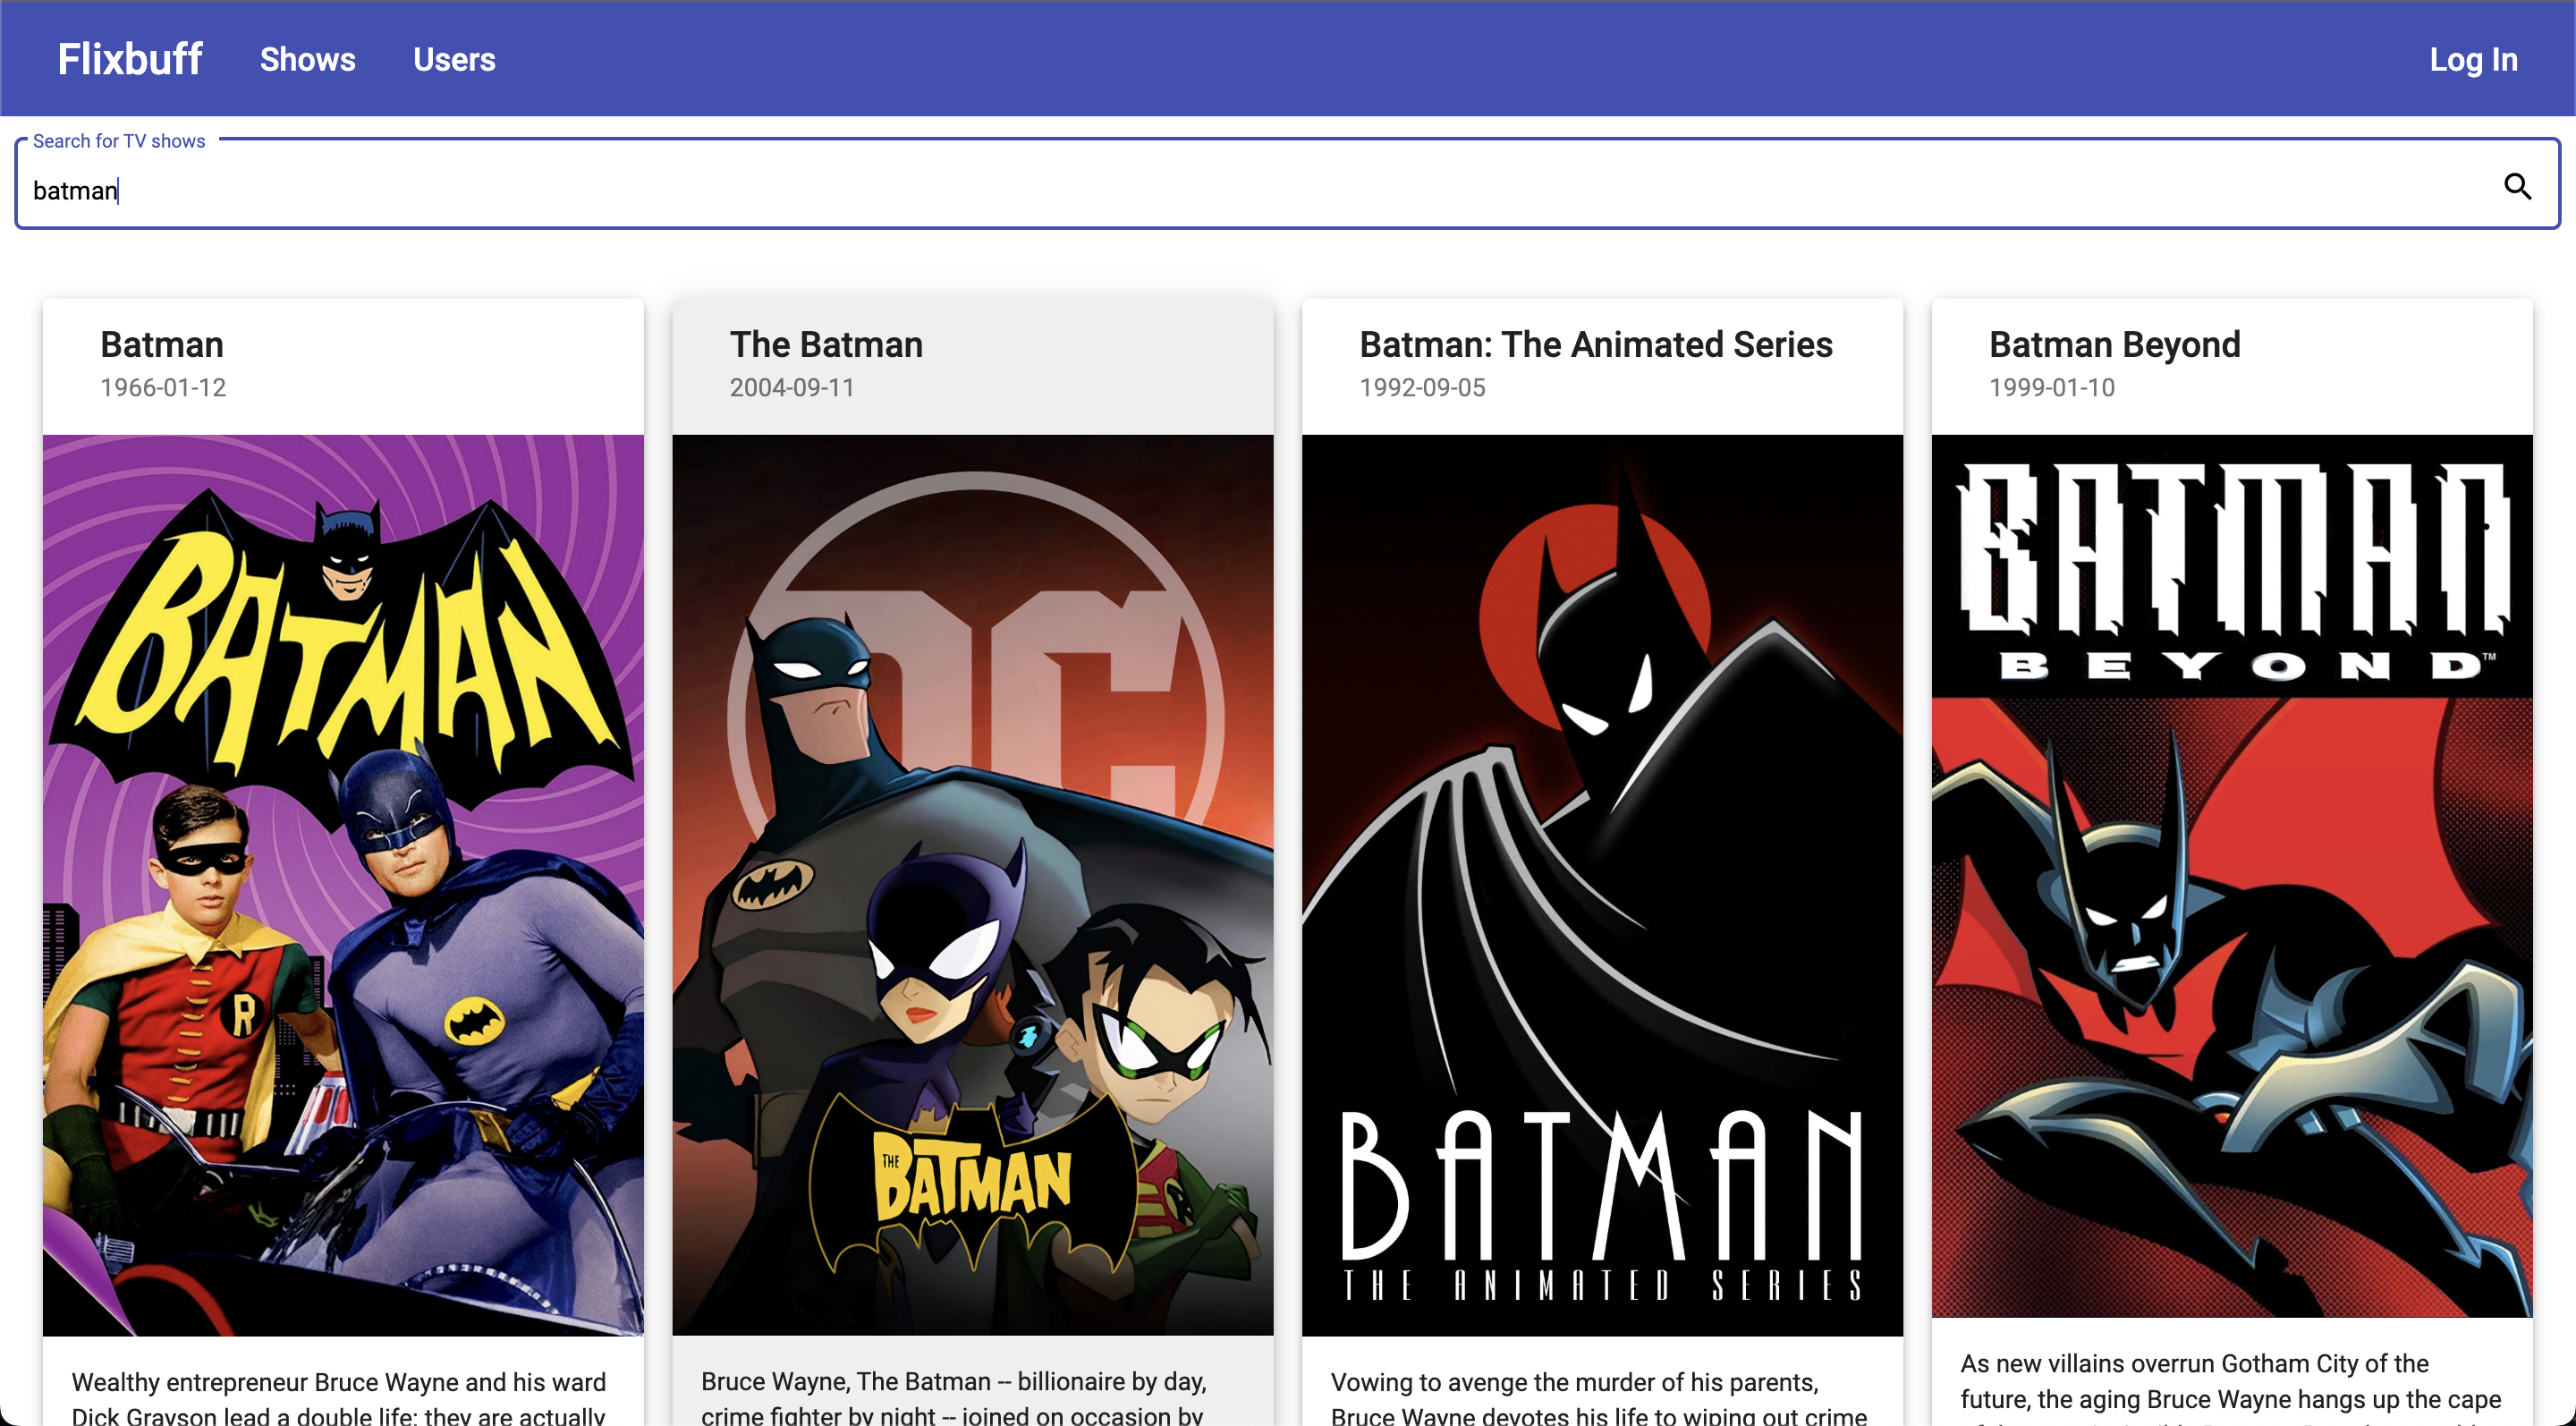
\includegraphics[scale=0.25]{img/show-list.png}
    \caption{ Lista de series con el nombre \textit{Batman} }\label{fig:show-list}
\end{figure}

Al igual que en la sección anterior, hacer click en una de las tarjetas te llevará a la vista de detalles de la serie.

\subsubsection{Detalles de una serie}
La vista de detalles de la serie nos muestra dos partes. \\

La primera parte es una cabecera con información de la serie, en la que, al igual que en la tarjeta, se podrán ver su
título, fecha de estreno, un pequeño resumen y una imagen de la misma.\\

La segunda parte está formada por la lista de sus temporadas, representadas en unas tarjetas expansibles, que al hacer
click sobre ellas, revelan más información sobre la misma.

\begin{figure}[H]
    \centering	
        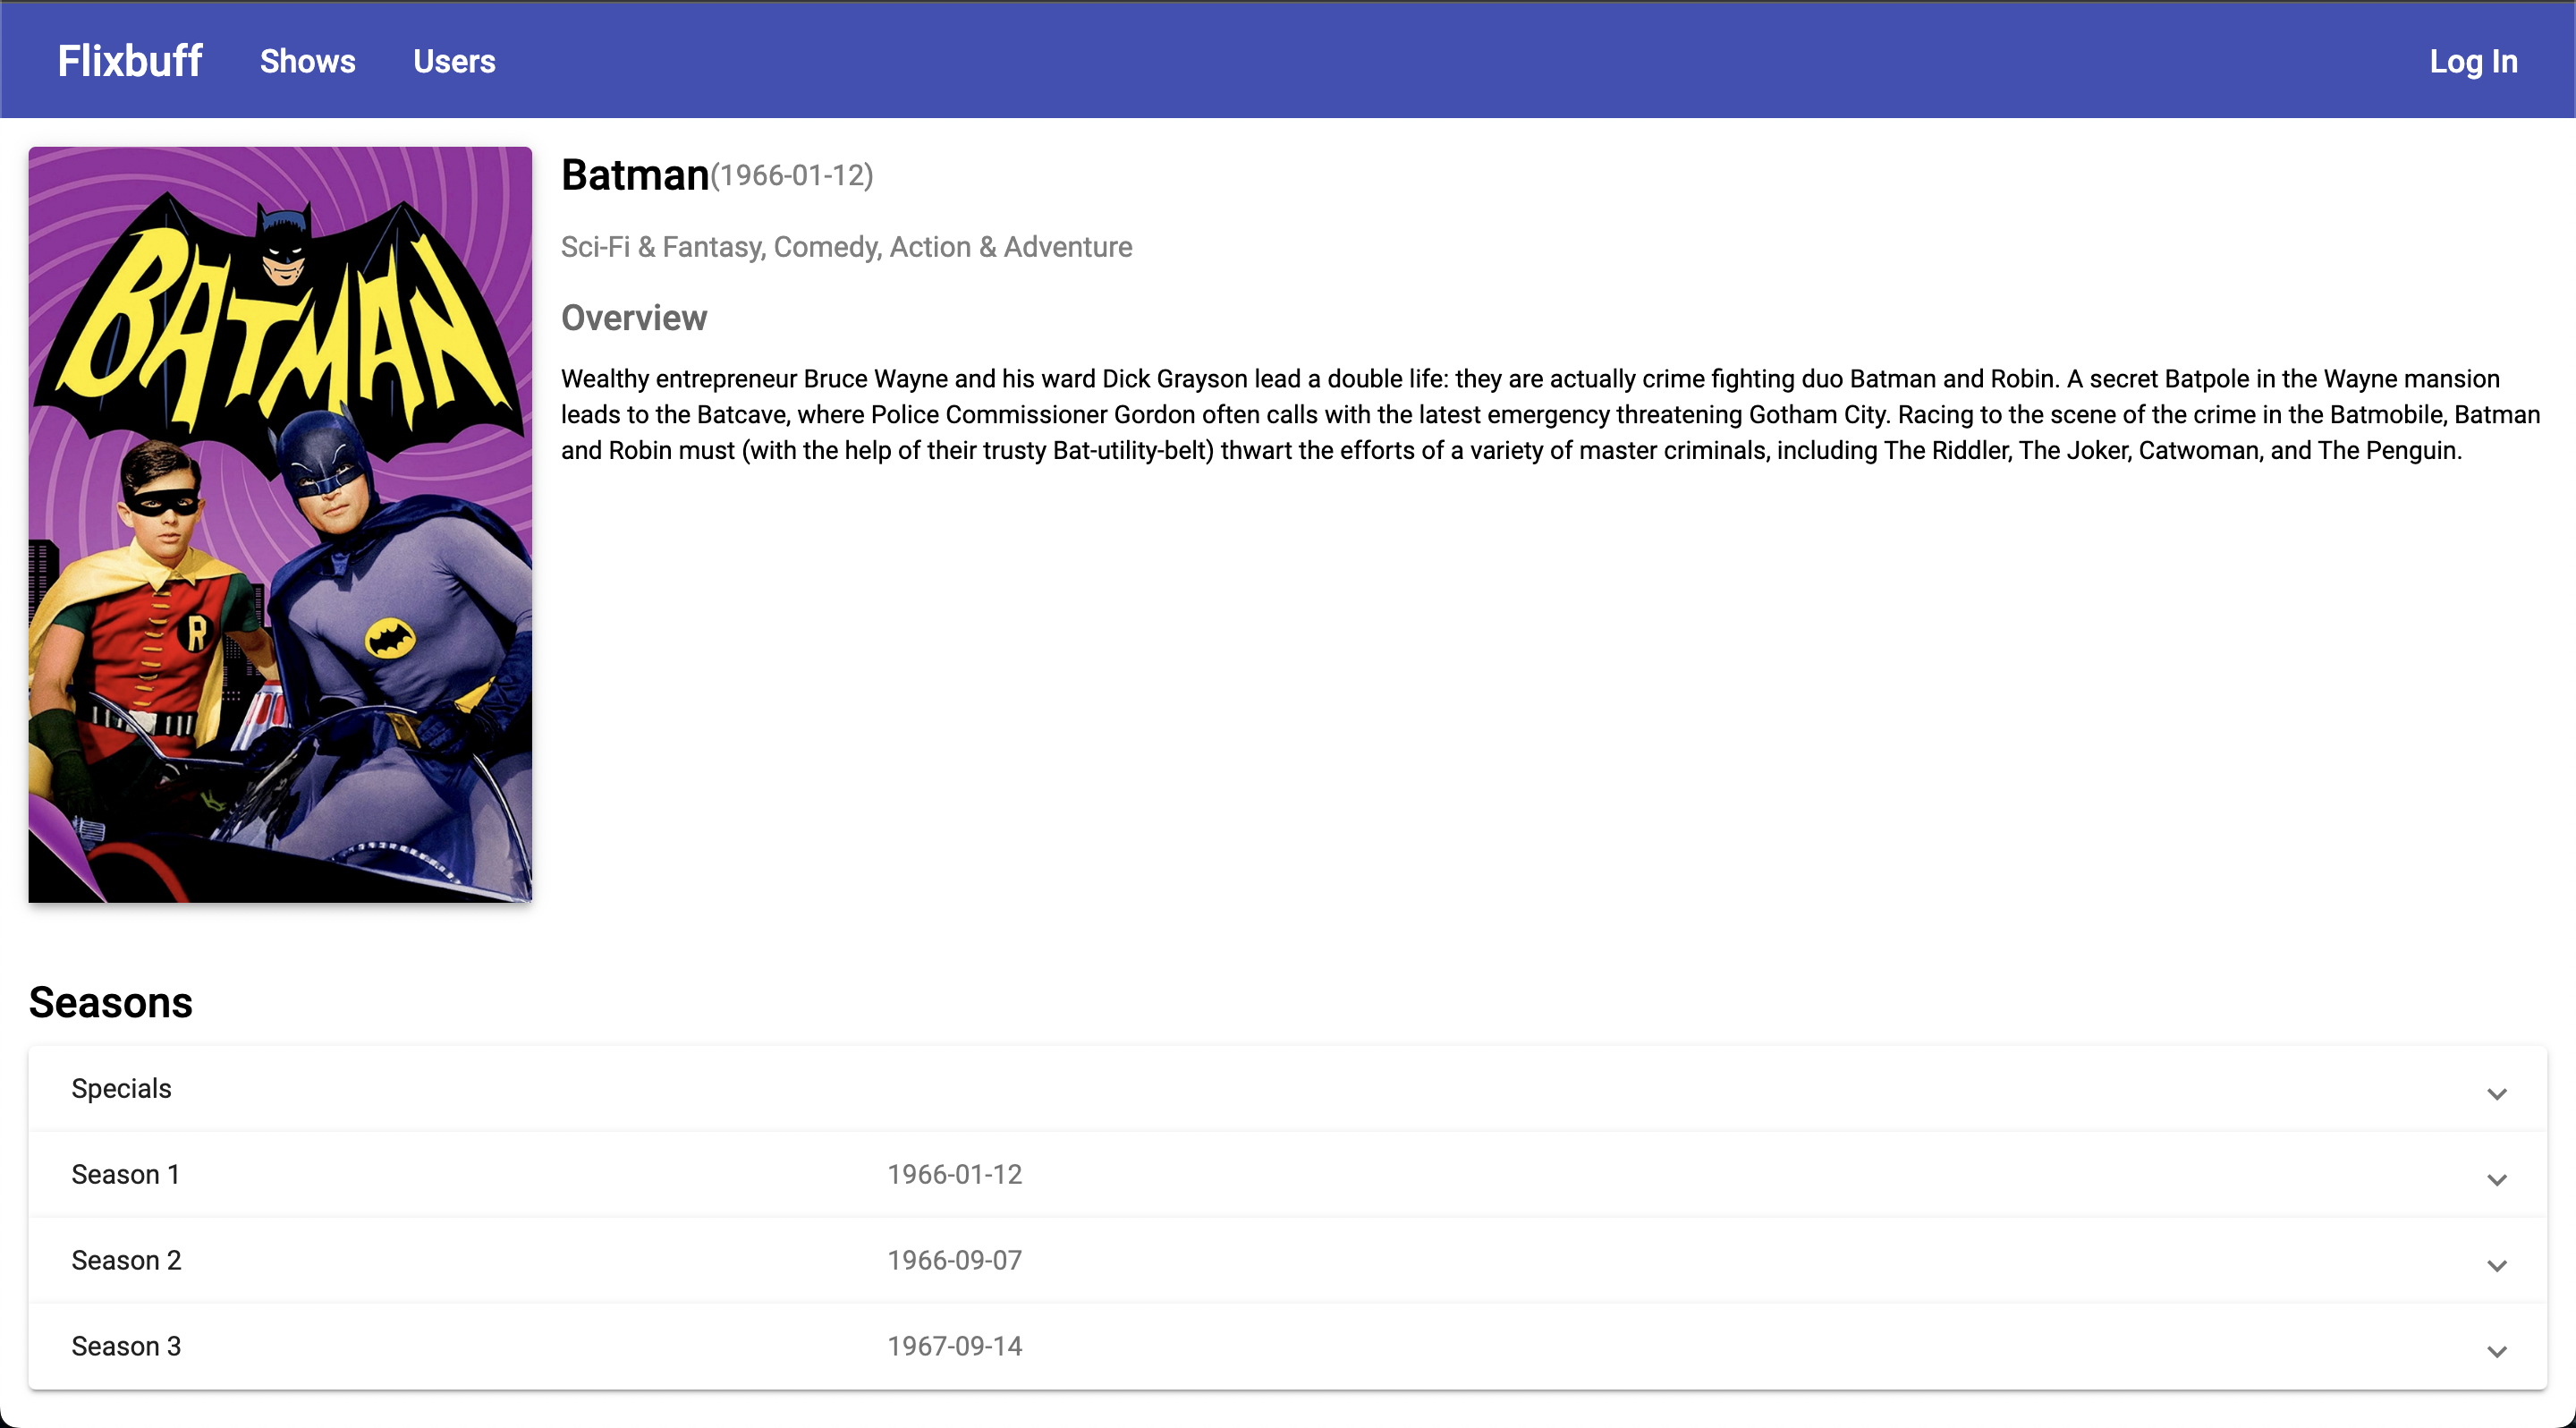
\includegraphics[scale=0.25]{img/show-details.png}
    \caption{ Detalles de la serie \textbf{Batman} }\label{fig:show-details}
\end{figure}

\begin{figure}[H]
    \centering	
        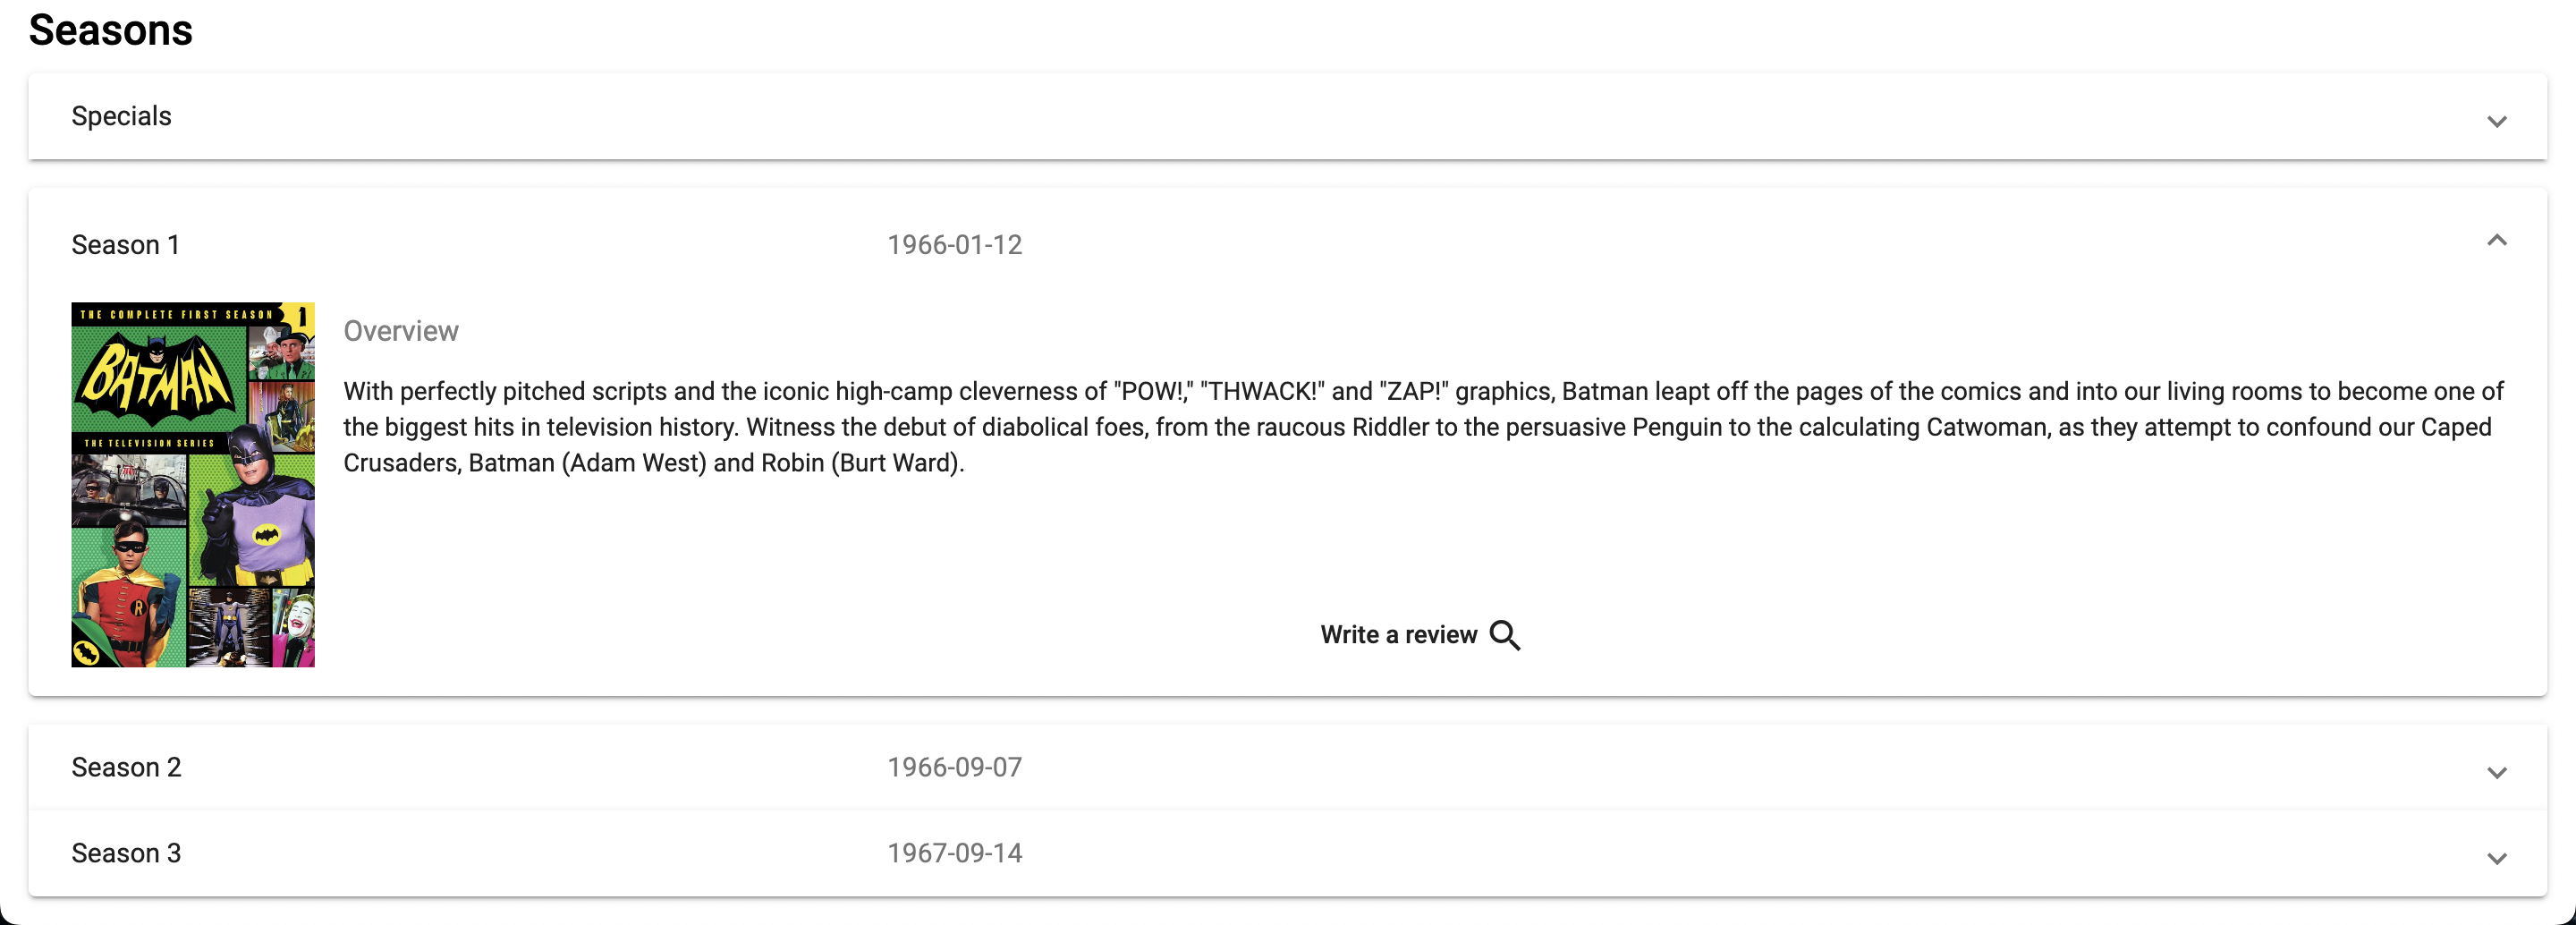
\includegraphics[scale=0.25]{img/expanded-season.png}
    \caption{ Lista de tarjetas de las temporadas de una serie }\label{fig:expanded-season}
\end{figure}

\subsubsection{Lista de usuarios}
Al igual que la lista de series, la lista de usuarios también se basa en una barra de búsqueda y unas tarjetas de
usuario. En este caso las tarjetas de usuario incluyen su nombre de perfil, el total de reseñas realizadas por el
usuario y el total de usuarios que le siguen. Haciendo click sobre ellas, navegas a la vista de detalles de ese
usuario.

\begin{figure}[H]
    \centering	
        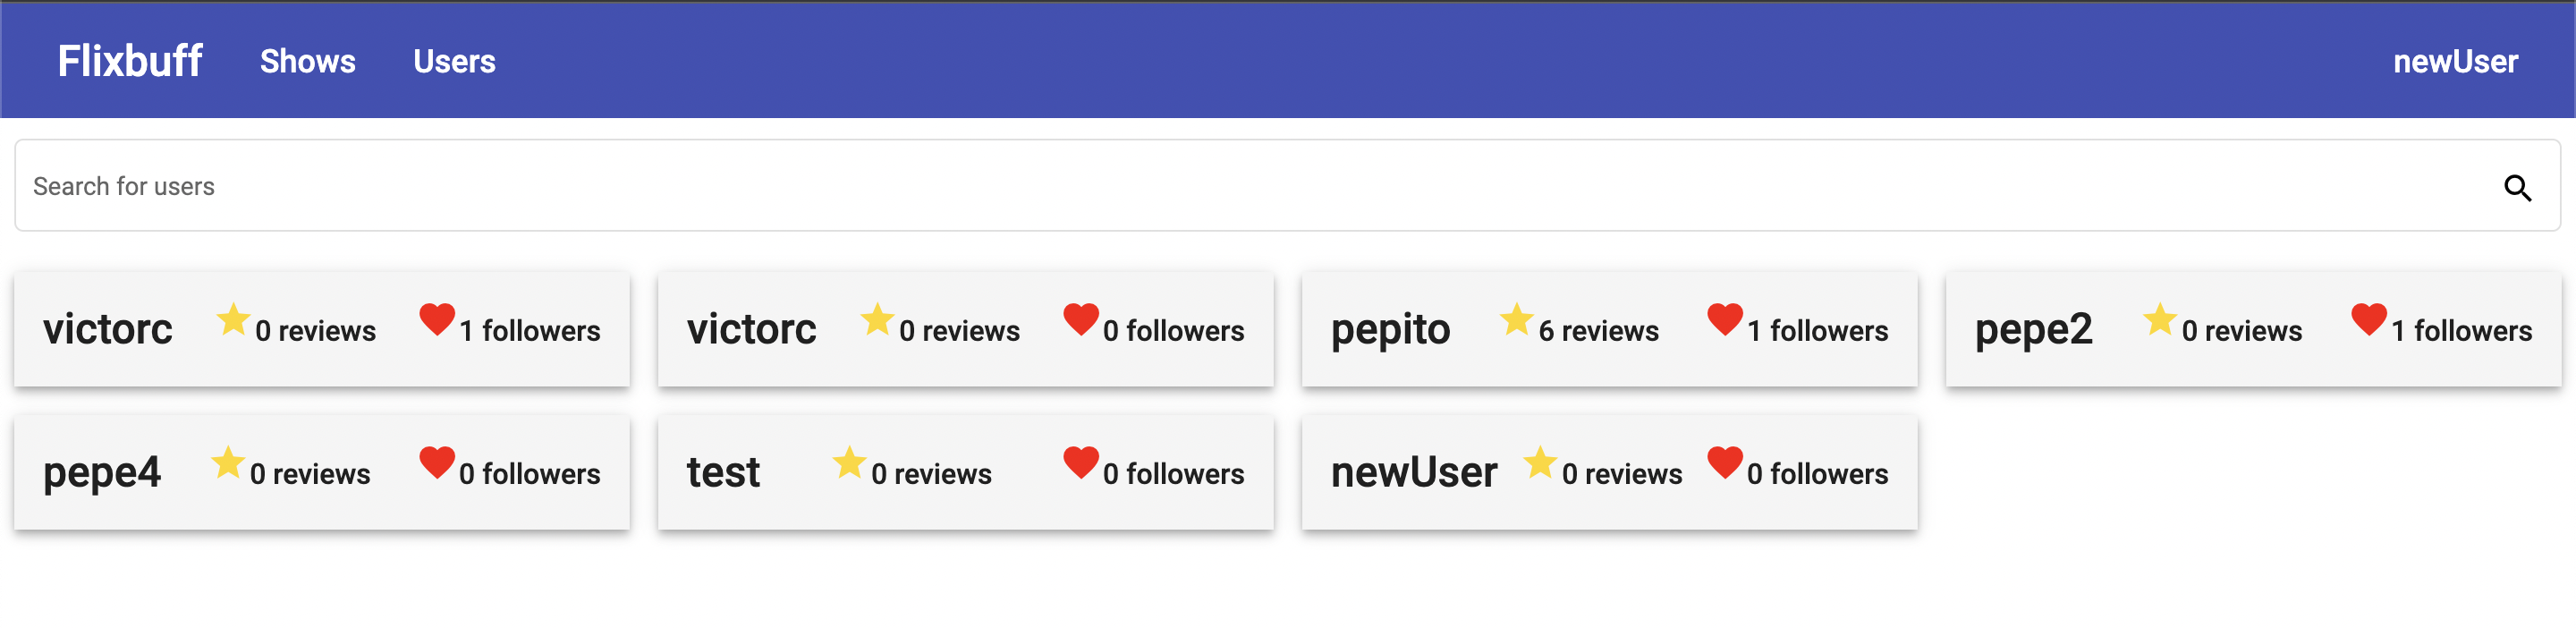
\includegraphics[scale=0.25]{img/user-list.png}
    \caption{ Lista de usuarios de la aplicación }\label{fig:user-list}
\end{figure}

\subsubsection{Detalles de un usuario}
La vista de detalles del usuario, muestra una rejilla de tarjetas, en las que se representan todas sus reseñas,
ordenadas de más a menos recientes.\\

En la esquina superior derecha, se muestra un botón de \textit{follow} a los usuarios logueados, para que puedan seguir
al usuario del que están viendo los detalles.

\begin{figure}[H]
    \centering	
        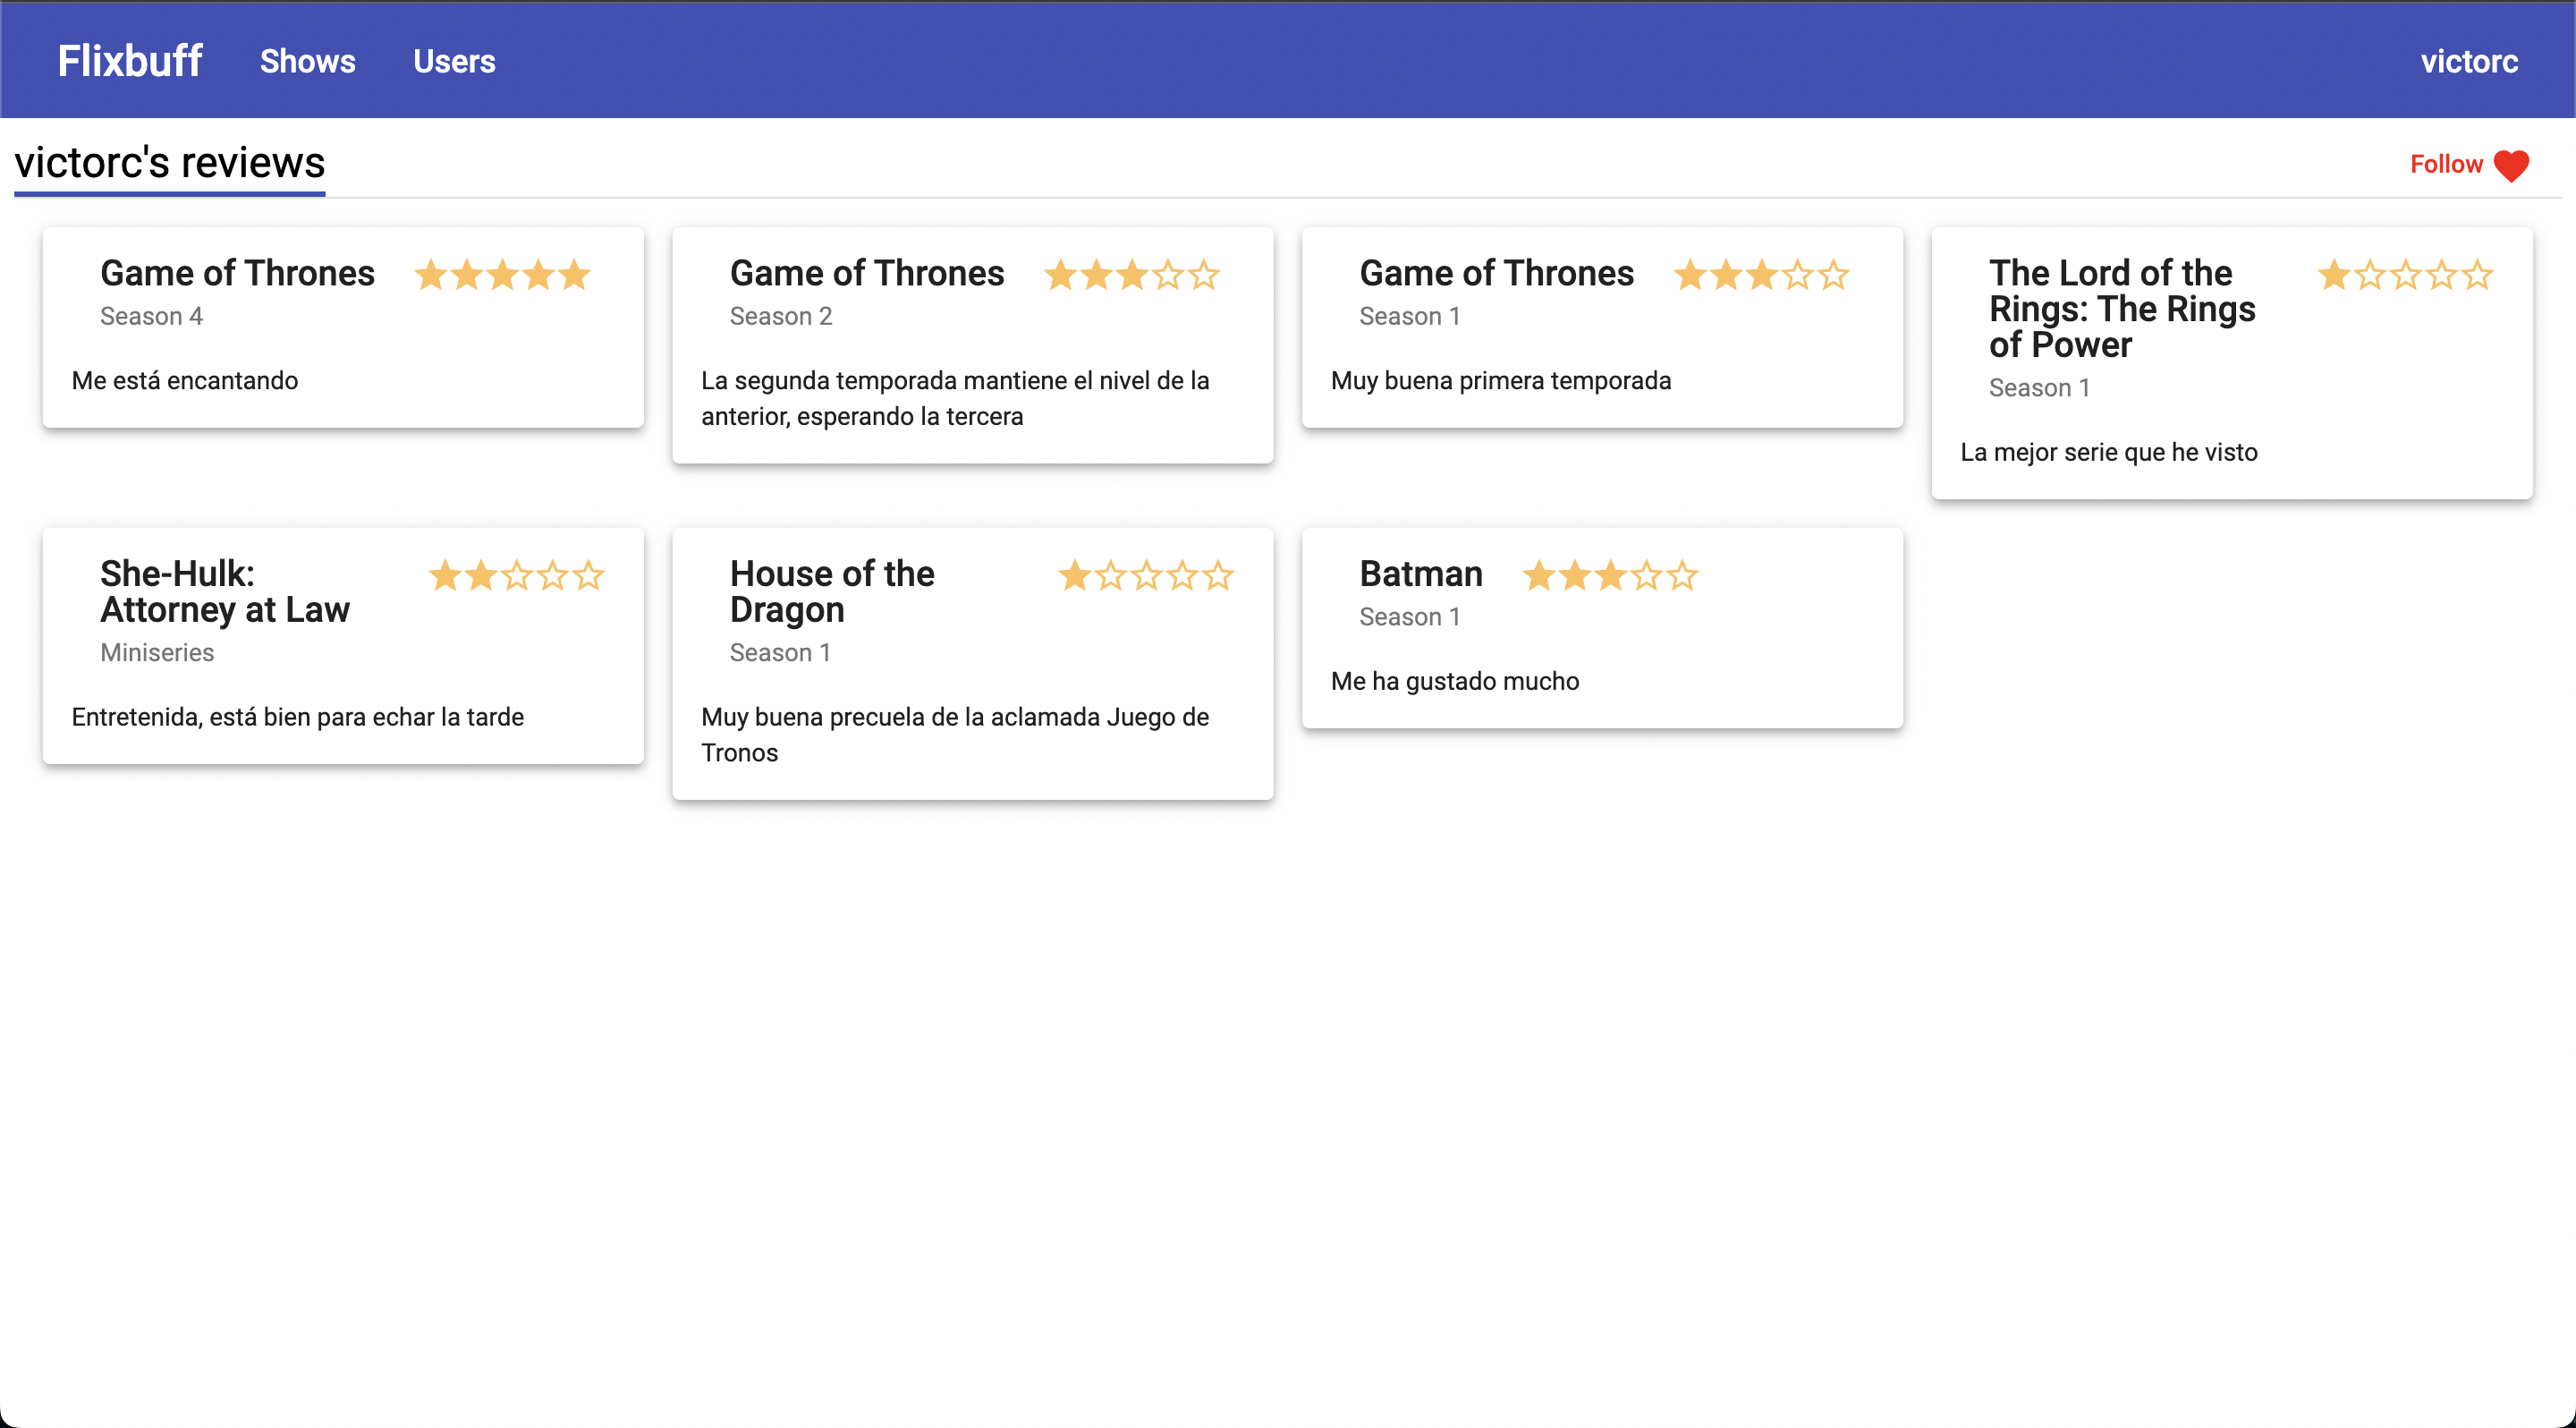
\includegraphics[scale=0.25]{img/user-details.png}
    \caption{ Detalles del usuario victorc }\label{fig:user-details}
\end{figure}

\section{Despliegue}\label{sec:despliegue}
Para el despliegue de la aplicación había infinidad de opciones en cuanto a servidores: montar un servidor en una
máquina de Ubuntu, \textit{AWS}\cite{aws}, \textit{Azure}\cite{azure}, etc.\\

Después de barajar las posibilidades hemos elegido \textit{Heroku}, una plataforma en la nube que nos permite montar un
servidor con nuestra aplicación, de forma muy sencilla e intuitiva, directamente desde nuestro repositorio en
\textit{GitHub}, permitiéndonos despliegues manuales o automáticos de cualquier rama del repositorio.\\

Para nuestra base de datos, hemos utilizado \textit{MongoAtlas}, de la que hablamos en secciones anteriores.

\subsection{Implementación del despliegue}
Hemos creado dos aplicaciones en la plataforma: una para servir la aplicación web y otra para la API.\\

Para desplegar el servidor, hemos necesitado instalar \textit{gunicorn}\cite{gunicorn}, que nos permite transformar
nuestra aplicación de \textit{flask} en un servidor HTTP. Además, hemos dado instrucciones a \textit{Heroku} a través de
un fichero \textit{Procfile} en el que se detalla cómo ejecutar el servidor con \textit{gunicorn}.

Por otra parte, para el despliegue del cliente, hemos creado un fichero \textit{server.js} que se ocupa de escuchar las
peticiones del puerto 8080 y devolverles los ficheros correspondientes. El resultado del despliegue se puede ver
\href{http://flixbuff-front.herokuapp.com/}{aquí}.\\

Al estar las aplicaciones dentro de subdirectorios en el repositorio, hemos utilizado un \textit{buildpack} para
\href{https://github.com/timanovsky/subdir-heroku-buildpack.git}{subdirectorios}, que nos permite establecer qué
subdirectorio de nuestro repositorio utilizar para el servidor, en lugar del repositorio completo.

\subsection{Costes del despliegue}\label{sec:costes-despliegue}
\subsubsection{Heroku}
\textit{Heroku} nos ofrece distintas \textit{tiers} de precios para alojar nuestra aplicación, desde una \textit{tier}
gratuita, hasta una \textit{tier} de altas prestaciones.\\

Dentro de cada \textit{tier} nos ofrece distintos \textit{dynos}, contenedores ligeros y aislados de Linux, en los que
se ejecuta tu aplicación. Cada uno de los distintos tipos de \textit{dyno}, tiene un precio distinto.

\begin{figure}[H]
    \centering	
        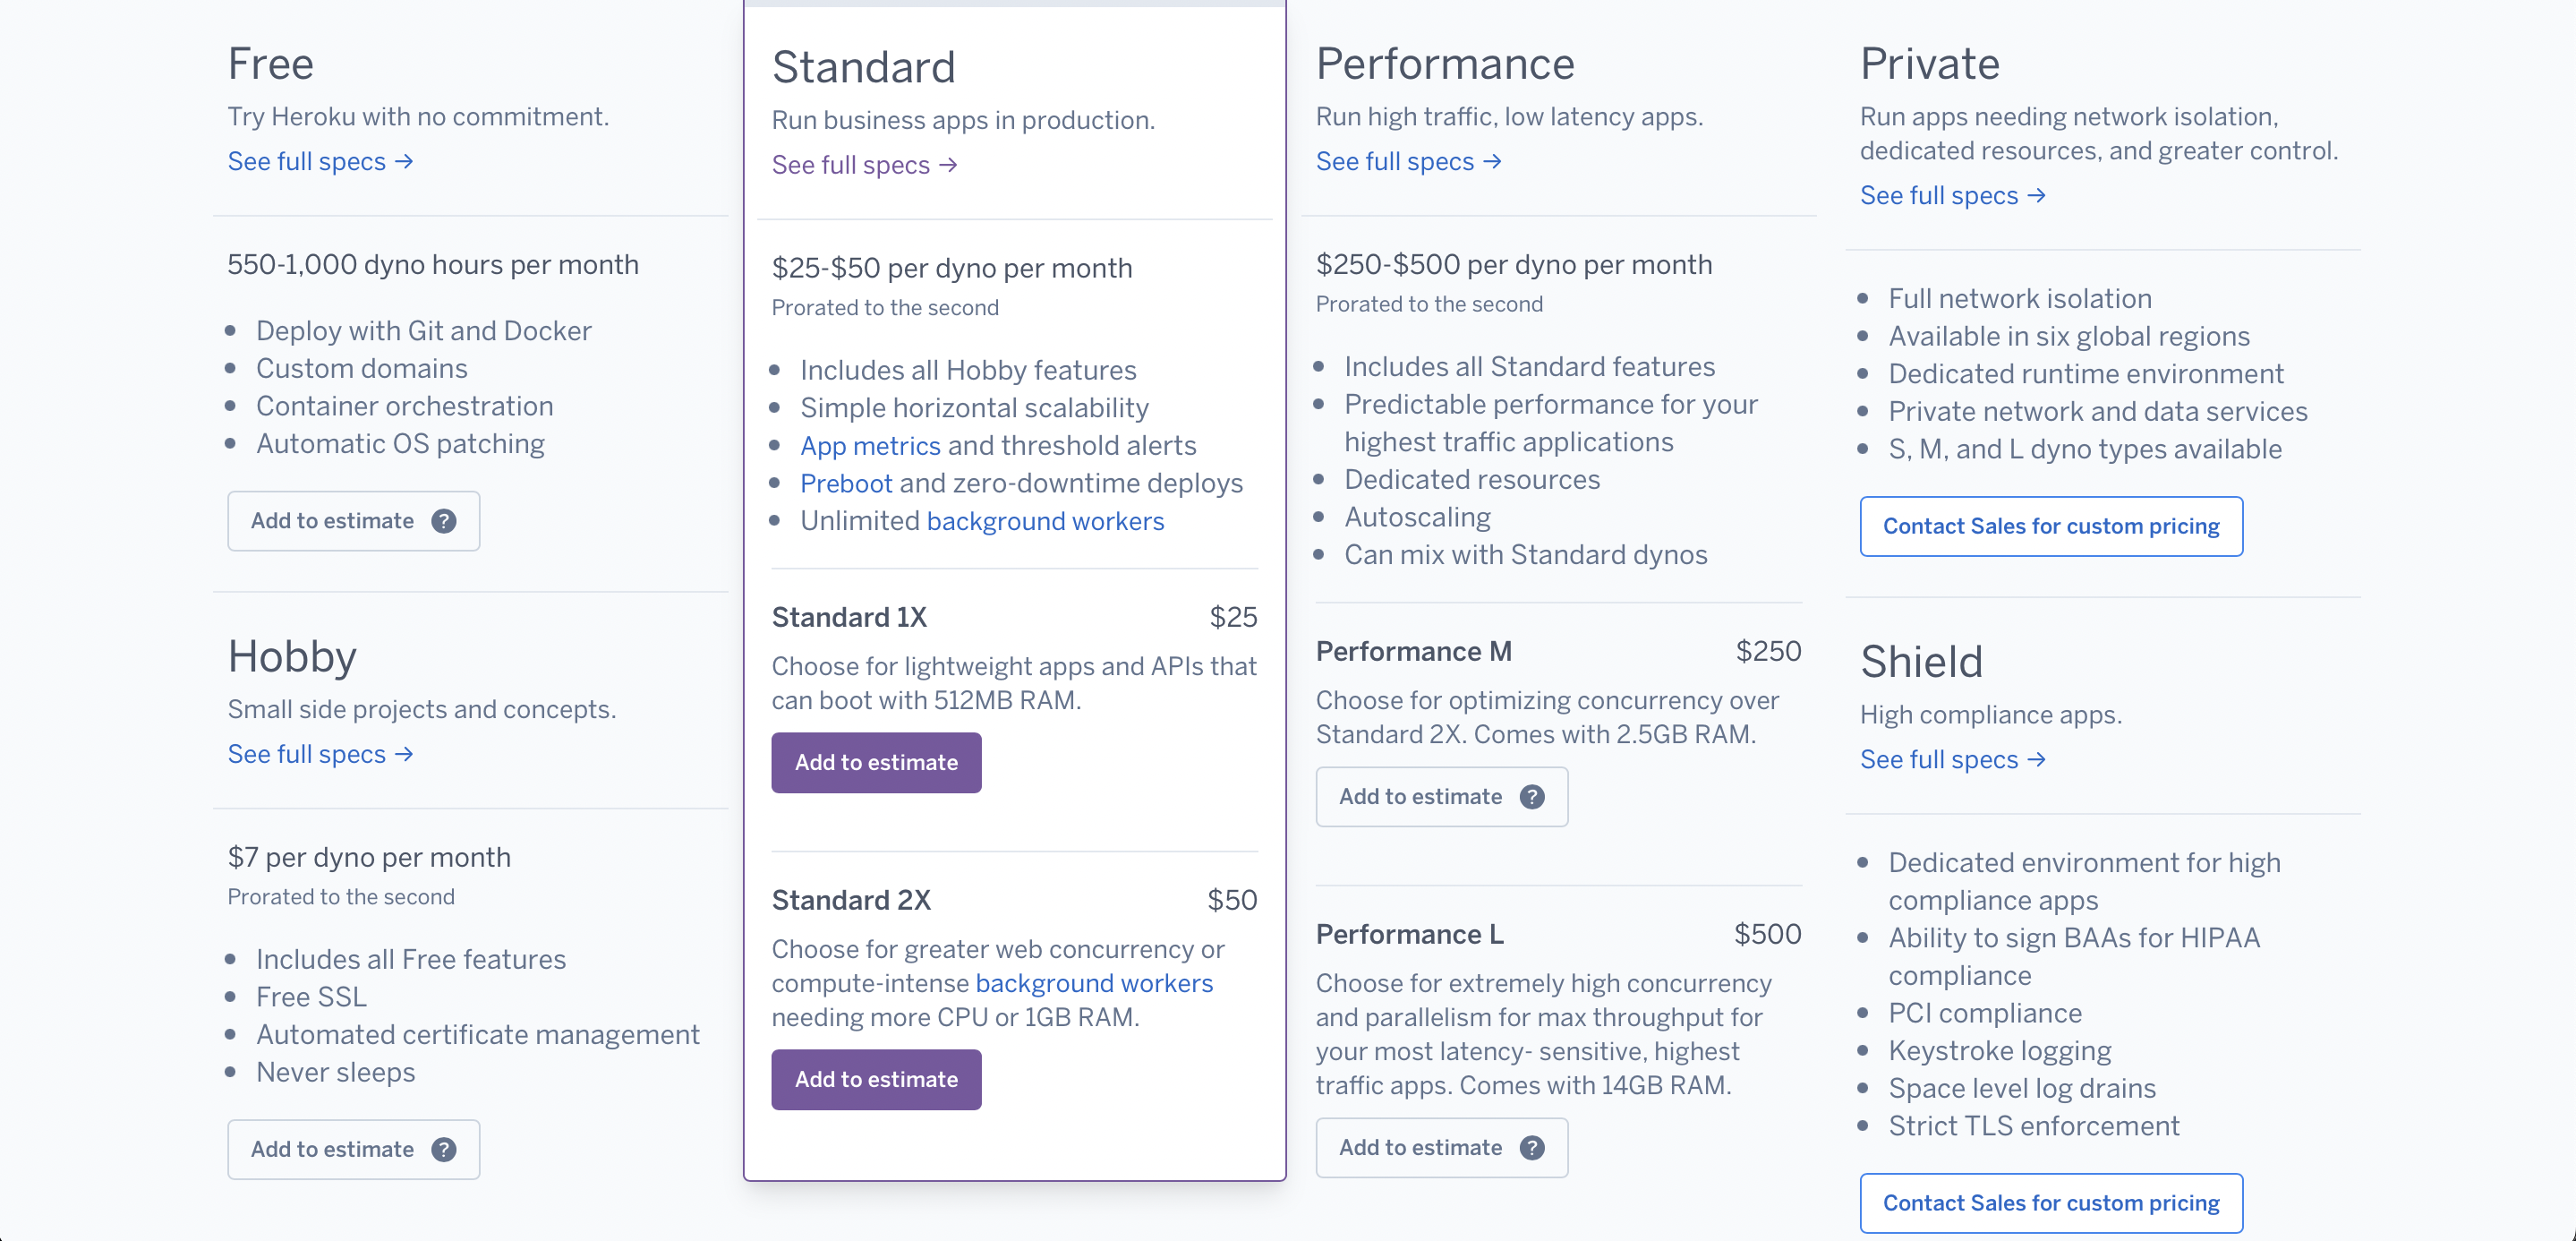
\includegraphics[scale=0.25]{img/heroku-tiers.png}
    \caption{ Precios de las \textit{tiers}/\textit{dynos} de \textit{Heroku} }\label{fig:heroku-tiers}
\end{figure}

En esta etapa del desarrollo del proyecto, elegiremos el \textit{tier} gratuito, ya que el proyecto aún está en
desarrollo.\\

Una de las ventajas de \textit{Heroku} es que nos permite fácilmente cambiar de \textit{tier} en el momento que
queramos, permitiéndonos escalar nuestra aplicación fácilmente.

\subsubsection{MongoAtlas}
Al igual que \textit{Heroku}, \textit{MongoAtlas} también nos ofrece diferentes planes y \textit{tiers}.\\

Cuenta con tres planes principales: \textit{serverless}, para aplicaciones con poco tráfico o simple almacenaje de
datos, \textit{dedicado}, el recomendado para aplicaciones en producción, y \textit{compartido}, para pruebas y 
aplicaciones en desarrollo.\\

Cada uno de los planes cuenta con diferentes \textit{tiers} de clústeres, cada uno con diferente precio y
prestaciones.\\

En nuestro caso, al igual que con el servidor de \textit{Heroku}, hemos optado por la opción gratuita, sabiendo que
podremos escalarla fácilmente desde la configuración de \textit{MongoAtlas}.

\begin{figure}[H]
    \centering	
        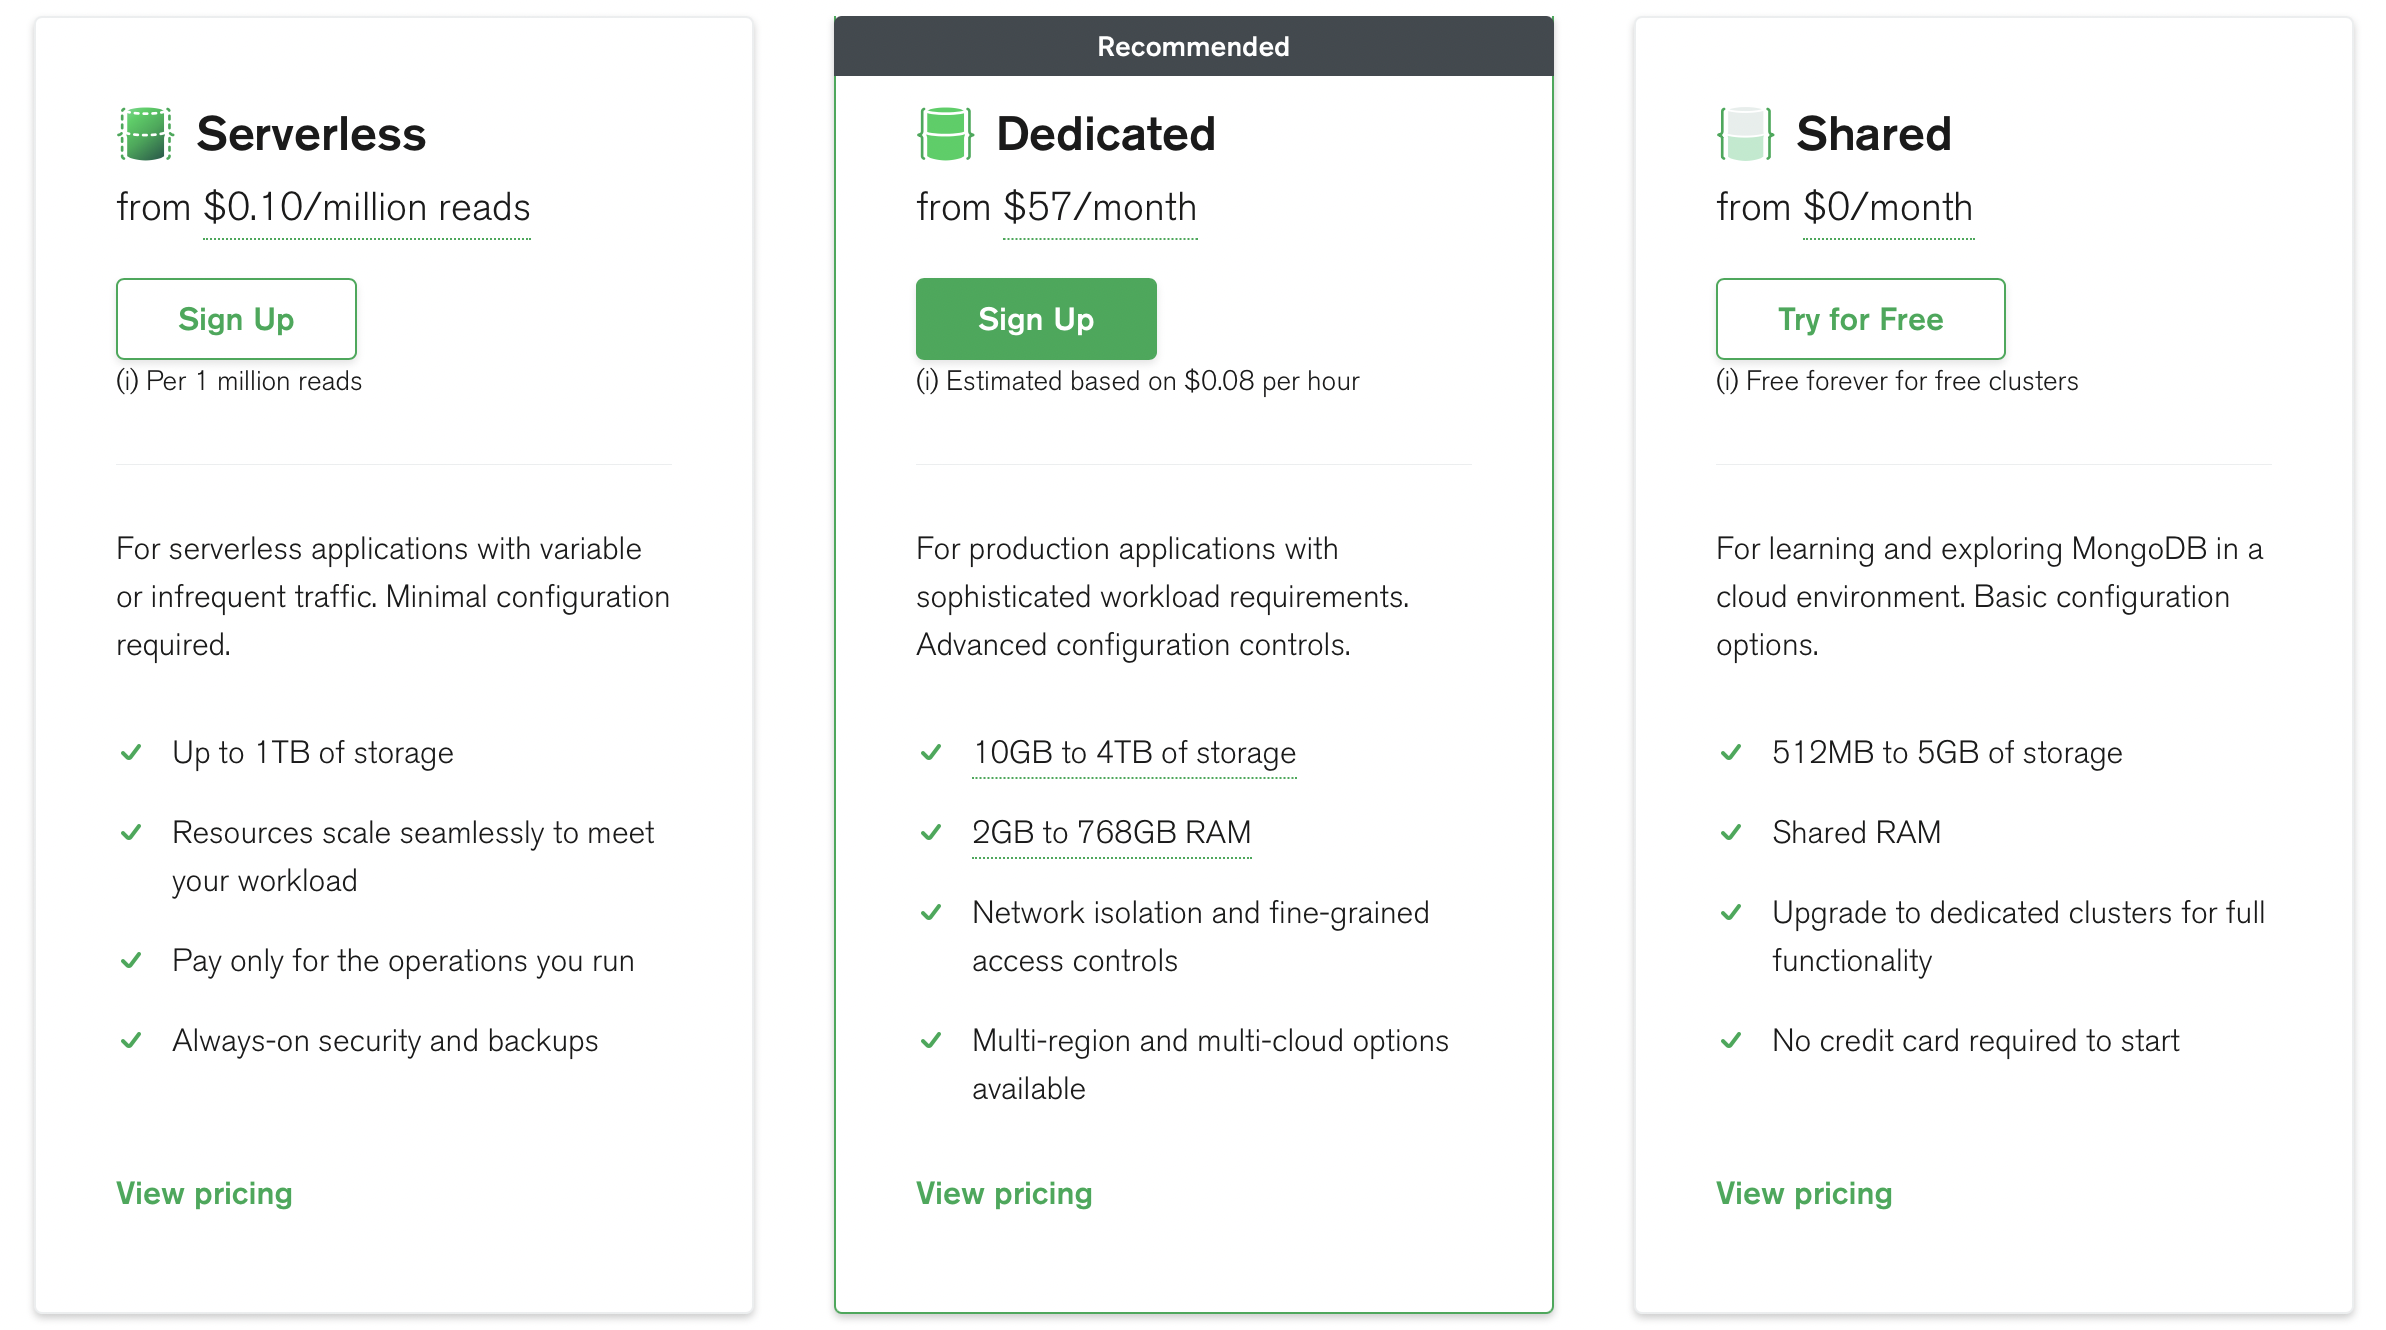
\includegraphics[scale=0.25]{img/mongo-plans.png}
    \caption{ Precios estimados de los distintos planes de \textit{MongoAtlas} }\label{fig:mongo-plans}
\end{figure}

\begin{figure}[H]
    \centering	
        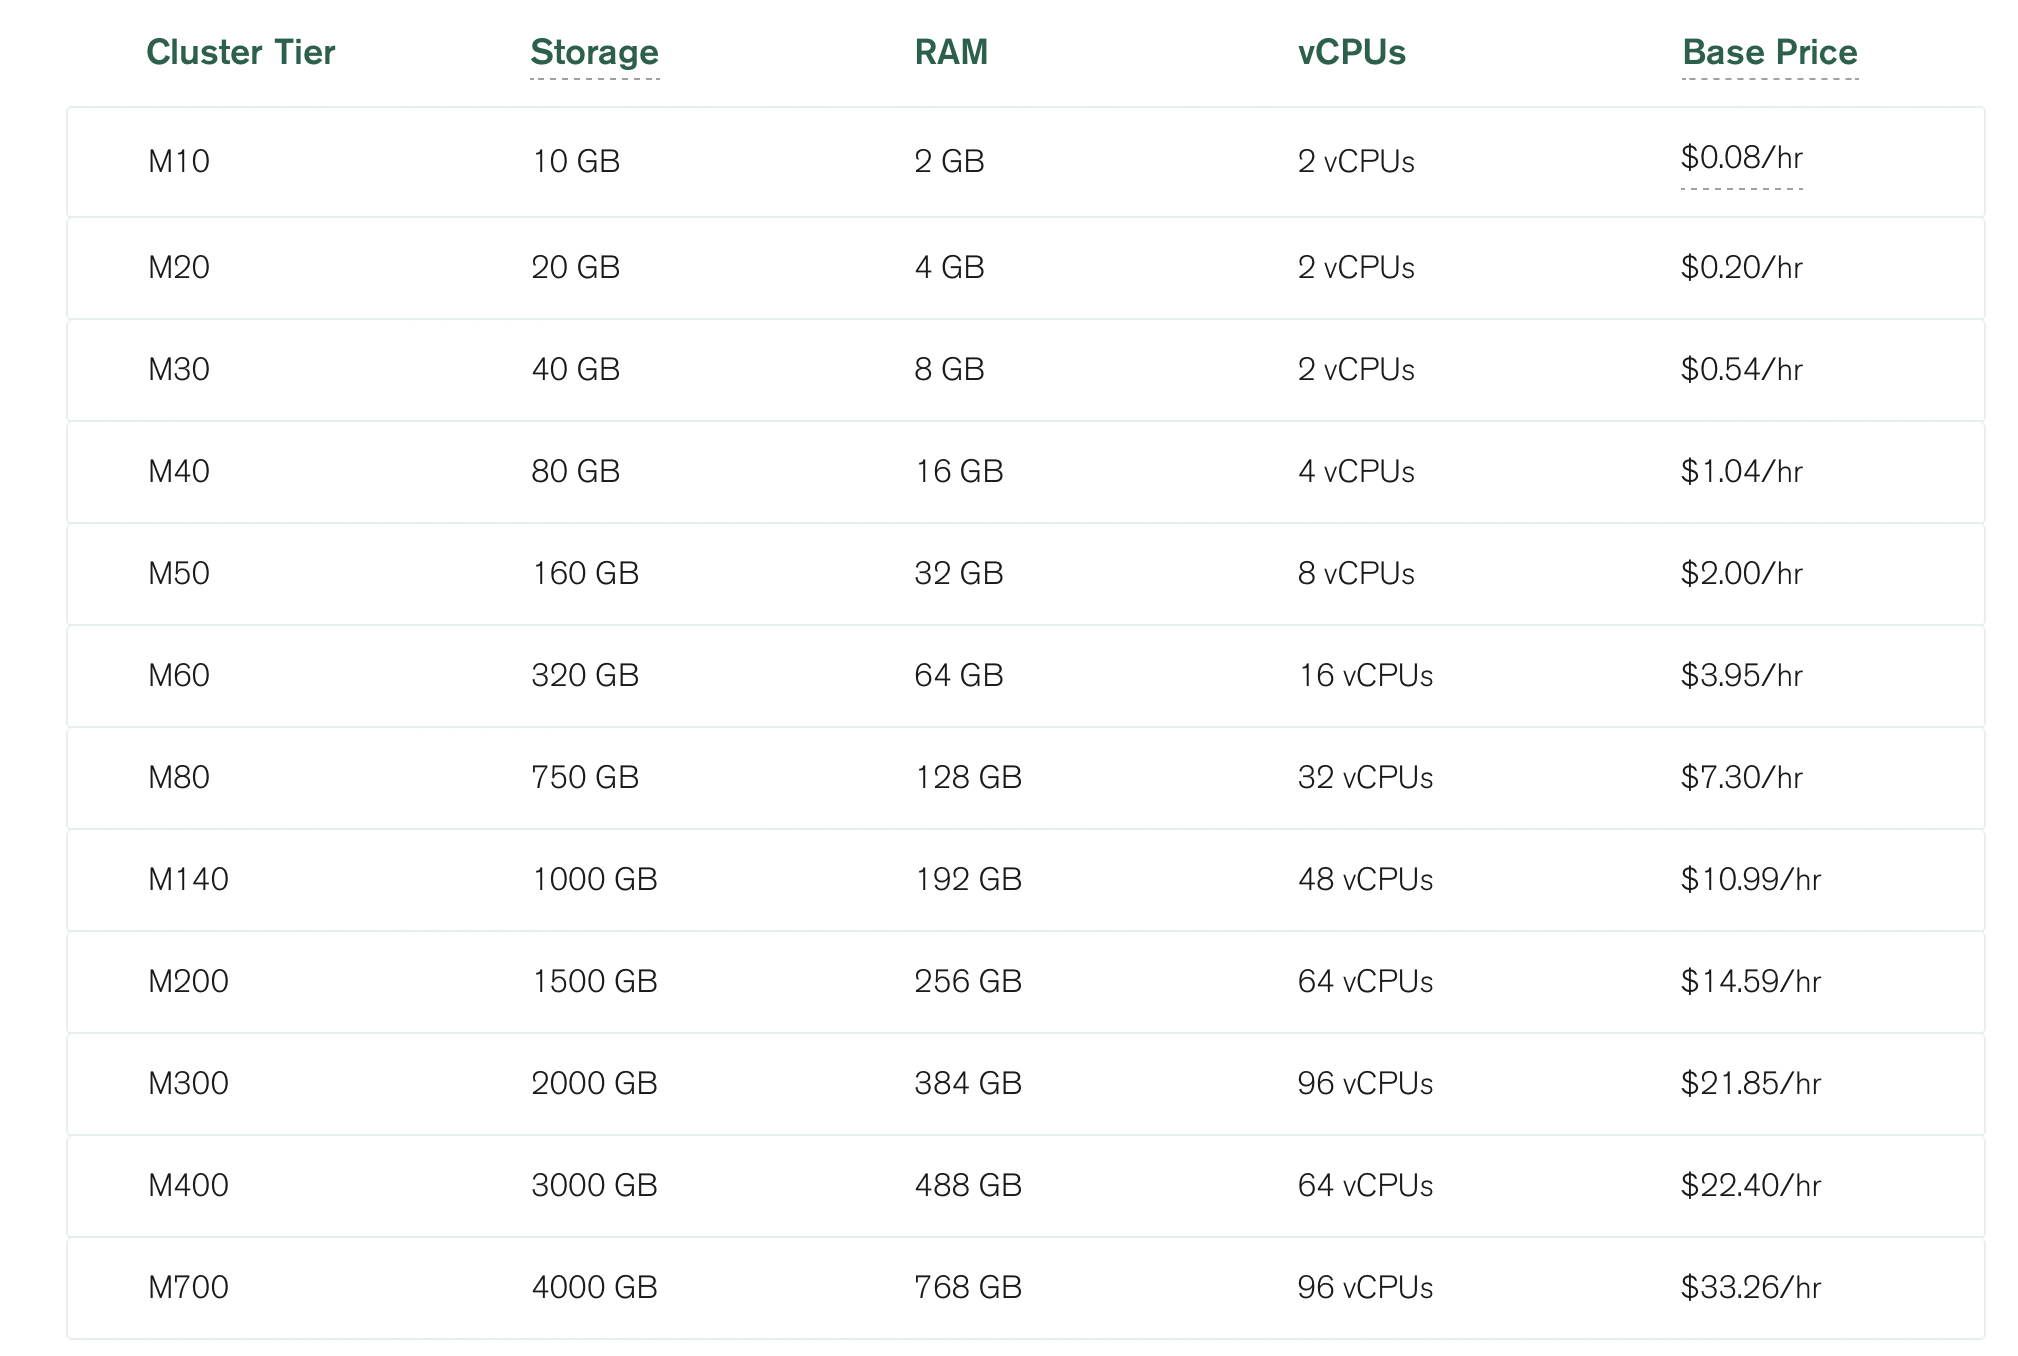
\includegraphics[scale=0.25]{img/mongo-tiers.png}
    \caption{ Precios de las \textit{tiers} de \textit{MongoAtlas} }\label{fig:mongo-tiers}
\end{figure}


	% Presupuesto

	% Conclusiones
	\chapter{Conclusiones y trabajos futuros}
\section{Conclusiones}
En este capítulo vamos a analizar el grado de cumplimiento de los objetivos definidos en el
\hyperref[sec:objetivo]{primer capítulo} y plantear las posibles lineas futuras de trabajo.\\

Los dos principales desafíos de este proyecto eran permitir a los usuarios crear reseñas de la serie que quieran y
permitirles seguir a otros usuarios para tener un rápido acceso a las reseñas de éstos. Ambos objetivos se han
conseguido en la aplicación web tal y como se refleja en la \hyperref[chap:implementación]{implementación}.\\

Esta nueva aplicación consigue con éxito satisfacer las necesidades \textit{seriéfilas} y sociales de los usuarios, que
se encontraban huérfanos de una plataforma en la que expresar su opiniones y leer las de los demás sobre sus series
favoritas.\\

En lo personal, este proyecto me ha servido para aprender y vivir la experiencia de realizar un proyecto de ingeniería
desde cero. Plantear los objetivos, estimar los costes y establecer y seguir una metodología de trabajo ágil, son
conocimientos que me aportarán mucho más valor como ingeniero en el campo profesional.

\section{Trabajos futuros}
En esta sección pretendo exponer posibles lineas de trabajo a seguir para sacar más valor a la solución encontrada:

\begin{itemize}
    \item Permitir a los usuarios personalizar su perfil, mejorar la UI/UX del cliente o dar soporte a aplicaciones
    móviles enriquecerían la experiencia de los usuarios, mejorando su relación con la aplicación y atrayendo a más
    gente a su uso.
    \item Dar soporte a películas permitiría a los usuarios tener todas sus reseñas en una misma aplicación.
    \item Ofrecer a empresas un servicio de pago de análisis de datos que les permita conocer los gustos de ciertos
    sectores de la población. De esta forma, se podrían financiar los costes de la aplicación sin necesidad de anuncios
    o cobro a los usuarios.
\end{itemize}


	% Trabajos futuros


	
	\newpage
	\bibliography{bibliography}
	\bibliographystyle{plain}

	% Apéndices
	\newpage
	\begin{appendices}
		\chapter{Personas}\label{chap:personas}
\section{Clara}

\begin{itemize}
  \item \textbf{Nombre y apellidos: } Clara Sánchez.
  \item \textbf{Nació en: } Reinosa.
  \item \textbf{Reside en: } Santander.
  \item \textbf{Edad: } 19.
  \item \textbf{Estado civil: } Soltera.
  \item \textbf{Estudia: } Magisterio infantil.
  \item \textbf{Rasgos de personalidad: } 
  \begin{itemize}
    \item Divertida.
    \item Carismática.
    \item Social.
  \end{itemize}
  \item \textbf{¿Cuáles son sus entornos?: } 
  \begin{itemize}
    \item Compañeros de clase y de la residencia de estudiantes.
    \item Amigos del pueblo.
    \item Su familia.
  \end{itemize}
  \item \textbf{¿Qué influencia su opinión?: } 
  \begin{itemize}
    \item Lo que piensan sus amigos.
    \item Lo que lee en las redes sociales.
  \end{itemize}
  \item \textbf{¿Cuál es su relación con la tecnología?} 
  \begin{itemize}
    \item Utiliza aplicaciones de ofimática con el ordenador para los trabajos de la universidad.
    \item Principalmente utiliza su dispositivo móvil y una tablet para los momentos de ocio.
  \end{itemize}
\end{itemize}

\section{Carlos}
\begin{itemize}
    \item \textbf{Nombre y apellidos: } Carlos Martín.
    \item \textbf{Nació en: } Santander.
    \item \textbf{Reside en: } Madrid.
    \item \textbf{Edad: } 27.
    \item \textbf{Estado civil: } Soltero.
    \item \textbf{Estudió: } Comunicación audiovisual.
    \item \textbf{Trabaja: } Ayudante de realizador en una cadena de televisión.
    \item \textbf{Rasgos de personalidad: } 
    \begin{itemize}
      \item Tranquilo.
      \item Culto.
      \item Serio.
    \end{itemize}
    \item \textbf{¿Cuáles son sus entornos?: } 
    \begin{itemize}
      \item Compañeros de trabajo.
      \item Amigos de su ciudad natal.
      \item Otros escritores amateurs.
    \end{itemize}
    \item \textbf{¿Qué influencia su opinión?: } 
    \begin{itemize}
      \item Las opiniones de gente que respeta.
      \item Lo que lee en revistas especializadas.
    \end{itemize}
    \item \textbf{¿Cuál es su relación con la tecnología?} 
  \begin{itemize}
    \item Está acostumbrado a usar el ordenador para trabajar.
    \item Suele usar su portatil para su afición de escritor. Se siente más cómodo que con el teléfono móvil.
  \end{itemize}
  \end{itemize}
	\end{appendices}
	
\end{document}

